\documentclass[11pt]{article}
\usepackage[T1]{fontenc}
\usepackage{lmodern}
\usepackage{amsmath,amssymb,amsthm,mathtools}
\usepackage[margin=1in]{geometry}
\usepackage{booktabs,array,graphicx}
\usepackage{microtype}
\usepackage{enumitem}
\usepackage{xurl}
\usepackage[svgnames]{xcolor}
\usepackage{hyperref}
\hypersetup{
  colorlinks=true,
  linkcolor=MidnightBlue,
  citecolor=MidnightBlue,
  urlcolor=MidnightBlue,
  pdftitle={Exact shared-link hopping and a homological carrier in strong-coupling SU(N) Hamiltonian lattice gauge theory},
  pdfauthor={Alexander Smith}
}
\setlist{itemsep=2pt,topsep=4pt}
\setlength{\emergencystretch}{2em}
\raggedbottom

\theoremstyle{plain}
\newtheorem{theorem}{Theorem}
\newtheorem{proposition}[theorem]{Proposition}
\newtheorem{lemma}[theorem]{Lemma}
\newtheorem{corollary}[theorem]{Corollary}
\theoremstyle{definition}
\newtheorem{reported}[theorem]{Reported computational result}
\newtheorem{conditional}[theorem]{Conditional corollary}
\newtheorem{conjecture}[theorem]{Conjecture}
\theoremstyle{remark}
\newtheorem{remark}[theorem]{Remark}

% Check labels remain in the source for registry validation but are suppressed
% in the typeset article; Section~\ref{sec:repro} explains how to recover them.
\newcommand{\chk}[1]{}

\newcommand{\CF}{C_F}
\newcommand{\dg}{^{\dagger}}

\begin{document}

\title{\bfseries Exact shared-link hopping and a homological carrier\\
in strong-coupling $SU(N)$ Hamiltonian lattice gauge theory}
\author{Alexander Smith\\ \small Independent Researcher}
\date{29 August 2026}
\maketitle

\begin{abstract}
\noindent
We study the Kogut--Susskind Hamiltonian for pure $SU(N)$ gauge theory on a
periodic cubic spatial lattice at strong coupling. In the normalised
charge-odd fundamental-plaquette sector, an explicit order-two Weingarten
calculation gives the exact coefficient of hopping between adjacent
plaquettes that share one link,
\[
  t_N=\frac{2N(N^2-4)}{(N^2-1)(2N^2-1)(4N^2-9)}>0,\qquad N\ge 3 .
\]
The oriented cellular boundary $B=\partial_2\dg$ fixes the corresponding local
geometry. Two premises that earlier versions carried as hypotheses---that the
retained external space is exactly the charge-odd one-plaquette shell, and
that shared-link routes exhaust second-order off-diagonal processes---are
proved here, from one classical Casimir-minimality fact and exhaustively
enumerated lattice combinatorics, so the global order-$u^2$ symbol
$t_Nu^2B(k)B(k)\dg$ is now a theorem within the standard degenerate
perturbation framework. Its spectrum is
$\{0,t_Nu^2q,t_Nu^2q\}$ up to a common scalar, with
$q=4\sum_j\sin^2(k_j/2)$, and its flat carrier
$\ker\partial_2$ has dimension $L^3+2$. A supplied $SU(3)$ two-cube
calculation reports the same coefficient channel by channel and localises the
cutoff dependence to one symmetry orbit; these finite-precision contractions
are corroboration, not an independent derivation. A later sealed cutoff-free
radius-two spectrum returns the coefficient without being asked for it: six of
the eleven eigenvalues of its second-order block are exact rationals, and the
outer pair straddles the central triple by exactly $2t_3=5/306$, in an
operator that made no shared-link truncation. Exact integer geometry also
gives the closed-cube shell
$A_1^{--}\oplus T_1^{+-}\oplus E^{--}$ with Gram eigenvalues $0,4,6$.

For comparison we solve the spectrum of a defined unsigned-incidence operator
in closed form. Identifying that operator with the complete charge-even linked
Hamiltonian requires a further derivation, because the vacuum-mediated route
must be accounted for. The organized upstream corpus records a cold exact
replay of the retained $SU(3)$ third-order chain, although that microscopic
replay is not bundled here. Fourth-order physical-kernel diagnostics remain
conditional; in particular, the retained checkpoints provably do not determine
the off-axis coefficient.
All results are finite-volume, finite-order statements in a projected
strong-coupling sector. No continuum glueball or Yang--Mills mass-gap claim is
made.
\end{abstract}

\section{Introduction}

Hamiltonian strong-coupling expansions organise lattice gauge dynamics around
the electric vacuum and its flux excitations~\cite{KS1975,KSS1976}. In three
spatial dimensions a fundamental plaquette excitation carries one of three face
orientations, and at second order neighbouring faces communicate through a
shared link, so the projected problem resembles a three-orbital tight-binding
model. The signs of those matrix elements are fixed by the orientation of the
plaquette boundary and by charge conjugation, and the resulting interference is
the central object here.

Flat bands generated by incidence or Gram matrices have a long history: local
topology and signed or line-graph constructions
~\cite{Eckmann1944,Sutherland1986,Mielke1991,Zaslavsky2010,Kollar2020},
compact localised states and their failure to span singular bands on a torus
~\cite{Bergman2008,RhimYang2019}, and supersymmetric incidence
factorisations~\cite{Roychowdhury2024} are all established. Closely related
closed-membrane structures also occur in two-form spin liquids
~\cite{ChungGingras2025}. A recent
classification of exactly flat bands protected by local graph
topology~\cite{Hazra2026} reaches extensive face-graph degeneracy from an
\emph{unoriented} face--vertex incidence, where rank--nullity alone gives
$|F|-|V|$ flat bands. That is a different mechanism from the one here, and the
difference is measurable: on the signed face--edge operator of
Section~\ref{sec:carrier} the corresponding index is exactly $0$ and bounds
nothing, while both kernels equal $L^3+2$ --- homology, not counting. It is
recorded as a distinction, not an identification. We do not claim that
incidence flatness, cellular compact localised states, or homological counting
are new in isolation.
\chk{the discrete index theorem gives 0 on the signed face-edge operator, bounding nothing}

The new dynamical content is local and exact. Starting from non-Abelian
$SU(N)$ Hamiltonian lattice gauge theory, the shared-link matrix element in the
charge-odd fundamental-plaquette sector factorises into a colour coefficient
and an oriented edge--face Gram entry. Representation theory fixes the former
and the cubical chain complex fixes the latter,
\[
  \begin{aligned}
    \text{colour dynamics}&\longrightarrow t_N,\\
    \text{cellular geometry}&\longrightarrow BB\dg .
  \end{aligned}
\]

\subsection*{What is proved, and what is conditional}

Seven mathematical statements are self-contained here; where an operator's
identification with a projected physical sector is conditional, that condition
is stated separately. Earlier editions carried three load-bearing prose
premises; this edition proves two of them --- the retained shell and
second-order process exhaustion (Lemmas~\ref{lem:shell}
and~\ref{lem:exhaust}, new here and flagged as such) --- which makes the
global second-order assembly a theorem (Theorem~\ref{thm:assembly}). The
third, the charge-even identification, remains a hypothesis and is argued in
Section~\ref{sec:scope}; the coverage appendix
(Appendix~\ref{app:coverage}) makes its unchecked status visible by
omission.

\begin{enumerate}\itemsep2pt
\item For every $N\ge3$ the shared-link channel weights are $d_\rho/N^2$,
  derived from the order-two Weingarten values
  (Theorem~\ref{thm:weingarten}). This was previously an isotropy
  \emph{hypothesis}, and everything in Section~\ref{sec:second} rests on it.
\item For every $N\ge3$ the exact adjacent shared-link matrix element has
  coefficient $t_N$ (Theorem~\ref{thm:allrank}). Its assembly into the global
  symbol $t_Nu^2BB\dg$ formerly assumed that the retained external range is
  exactly the charge-odd one-plaquette shell and that one-shared-link
  processes exhaust the second-order off-diagonal intermediates; both are
  now proved (Lemmas~\ref{lem:shell} and~\ref{lem:exhaust}), so the
  assembly is Theorem~\ref{thm:assembly}, resting on one classical
  Casimir-minimality input and machine-enumerated finite combinatorics.
\item The Bloch spectrum of $BB\dg$ is $\{0,q,q\}$ (Theorem~\ref{thm:fact}),
  and on the periodic $L^3$ complex the zero-mode count is $L^3+2$
  (Theorem~\ref{thm:carrier}). The two are the same statement, by a sum rule
  over the momentum grid (Theorem~\ref{thm:bridge}).
\item\label{item:cutoff} The truncation that keeps only the singlet and $\Lambda^2F$ routes
  projects the hopping to $w_{\Lambda^2F}-w_{\mathbf 1}=-1/12$, and what it
  omits is $w_{\mathrm{Sym}^2F}-w_{\mathrm{Adj}}=14/153$; the two sum to
  $t_3$ (Corollary~\ref{cor:cutoff}). This is arithmetic on
  \eqref{eq:w} and needs no input beyond Theorem~\ref{thm:weingarten}.
\item The defined unsigned-incidence comparison operator has the cubic
  $\mu(\mu-p)^2=4\hat a_1\hat a_2\hat a_3$ with $p+q=12$
  (Theorem~\ref{thm:evencubic}); its range is exactly $[-4,12]$, the top
  attained only at $\Gamma$ and the floor on the three planes $k_j=\pi$, triple
  only at $R$ (Proposition~\ref{prop:evenrange}). Conditional on identifying
  this comparison operator with the complete linked charge-even symbol, its
  $\Gamma$-point splitting is $12t_{r,+}$
  (Proposition~\ref{prop:evengamma}). That identification is not derived here;
  the vacuum-mediated all-pairs term must first be reorganised or cancelled.
\item On the closed cube surface the charge-odd shell is
  $A_1^{--}\oplus T_1^{+-}\oplus E^{--}$, with $G$-eigenvalues $0,4,6$; the
  labels follow from the rotation action rather than being assigned, the
  $A_1^{--}$ level is the fundamental class of $S^2$, and it sits at the scalar
  for every hopping coefficient (Proposition~\ref{prop:cube}). This is integer
  linear algebra and takes no input from any delivery.
\item The retained $\Gamma$/axis corpus cannot identify the disputed
  fourth-order off-axis coefficient (Theorem~\ref{thm:obstruction}), and an
  explicit second witness exhibits the non-identifiability by construction
  (Proposition~\ref{prop:witness}).
\end{enumerate}

Three families of statements depend on computational artifacts outside this
compact edition. Their raw class contractions, symbolic history certificates
and microscopic rank-sweep artifacts are not bundled here, and repeated
assertions in synthesis documents are not treated as independent
reproductions. The organized upstream authority corpus does record a cold exact
$251/251$ replay for the retained third-order operator chain; that is stronger
than an unchecked delivery, but it is still cited here as external
computational evidence because this release does not replay the raw chain.

\begin{enumerate}\setcounter{enumi}{7}\itemsep2pt
\item A supplied two-cube delivery reports six link-irrep channel
  coefficients at $N=3$, as rational reconstructions of finite-precision
  contractions. Conditional on those six numbers, they are the four
  fusion-channel weights individually --- channel by channel and not merely in
  the sum (Reported result~\ref{rep:census}) --- and the $\mathcal B=4$ truncation of
  that space retains exactly the adjacent shared-link channels the published
  link cutoff of item~\ref{item:cutoff} retains, so the two land on the same
  projected hopping --- the same channels, not the same scheme. Conditional on the delivered diagonals, the symmetry
  analysis of Proposition~\ref{prop:orbit} applies to them: the orbit structure
  itself is exact and takes no delivered input.
  The $\mathcal B=6$ two-cube build was not reproduced here.
\item\label{item:domino} For $SU(3)$, the frozen upstream corpus records that
  all candidate third-order lifter classes vanish and gives the scalar and
  shared-link coefficients of Section~\ref{sec:su3}. The census is three
  lifter classes evaluated over $32$ five-trace numerator patterns each, $96$
  contractions in total, within a retained chain that passed $251/251$ cold
  exact gates upstream. This compact verifier checks the resulting rational
  assembly but not those microscopic contractions. If the census is exhaustive
  and the linked operator ledger complete, the effective Hamiltonian stays in
  the incidence algebra through order $u^3$.
\item Supplied ledgers report the all-rank cube formula
  $\alpha_N=640/[N(N^2-1)^3]$ and its equality with the complete axial
  coefficient for $N=3,\dots,12$. Conditional on those calculations, the
  $SU(3)$ carrier acquires nonzero axial dispersion at order $u^4$. The
  complete off-axis operator remains open --- and by
  Theorem~\ref{thm:obstruction} it cannot be closed by any $\Gamma$ or axial
  datum.
\item A sealed cutoff-free radius-two spectrum
  (Section~\ref{sec:radius2}) is bundled with this edition, pinned by
  SHA-256. Its second-order block contains a rational sub-block whose
  splitting is exactly $2t_3$, its fourth- and fifth-order nested increments
  agree with independent weak-coupling intercepts, and its fifth-order seed
  object is a matrix, not a scalar. All of it is finite-precision and
  reported at stated tolerances; the exact-arithmetic identifications it
  corroborates are checked separately.
\end{enumerate}

These statements concern the effective Hamiltonian projected to the degenerate
one-plaquette manifold. Virtual multi-plaquette states are retained in the
resolvents, but the external spectral problem is not the full gauge-theory
Hilbert space. At $k=0$ the three incidence branches touch and the
finite-volume separation collapses as $L^{-2}$. Nothing below proves
convergence of the strong-coupling series, persistence under unrestricted
higher-order operators, identification with the lightest physical glueball, or
a continuum mass gap.

\section{Hamiltonian and projected sector}

Let $\Lambda_L=(\mathbb{Z}/L\mathbb{Z})^3$, $L\ge3$, be a cubic spatial
lattice with periodic boundary conditions. In units of the electric coupling
the Kogut--Susskind Hamiltonian is
\begin{equation}
  H_\beta=\tfrac12\sum_\ell C_2(\ell)
  +\beta_N\sum_p\Bigl(1-\tfrac1N\operatorname{Re}\operatorname{Tr}U_p\Bigr).
\end{equation}
Dropping the additive constant,
\begin{equation}\label{eq:H}
  H=H_E-uV,\qquad V=\sum_p(\chi_p+\bar\chi_p),\qquad u=\frac{\beta_N}{2N},
\end{equation}
with $\chi_p=\operatorname{Tr}U_p$. For $SU(3)$, $u=\beta_3/6$. The
definition $u=\beta_N/(2N)$, not the $SU(3)$-specific equality, is the
all-rank convention; the archived line $Y=2\beta/3=4u$ is a definition-label
erratum and the printed coefficients are already in $u$. Reading it as a
coordinate would demand dividing the order-$r$ coefficient by $4^r$, which
misses the printed tables by exactly $16$ at $u^2$ and $64$ at $u^3$.
\chk{the printed towers are canonical-u: 4*Delta(3u/2) reproduces them verbatim}
\chk{the 4**r rescaling breaks the bridge: order 2 off by 16, order 3 by 64}

All quoted excitation energies use the linked, vacuum-subtracted operator
$H_{\mathrm{exc}}(u)=H(u)-E_{\mathrm{vac}}(u)I$. This changes only the scalar
ledger; incidence hopping and carrier shape are unaffected.

The electric vacuum $|0\rangle$ carries the trivial representation on every
link. For $N\ge3$ the normalised one-plaquette states of definite charge
conjugation are
\begin{equation}\label{eq:states}
  |p,\pm\rangle=\frac{\chi_p\pm\bar\chi_p}{\sqrt2}\,|0\rangle ,
\end{equation}
of unit norm by character orthogonality. Each of the four boundary links
carries the fundamental or antifundamental representation, so
\begin{equation}\label{eq:EF}
  E_{F,N}=4\Bigl(\tfrac12 \CF\Bigr)=2\CF=\frac{N^2-1}{N},
  \qquad \CF=\frac{N^2-1}{2N}.
\end{equation}
This external energy is the input to the resolvent denominators of
Section~\ref{sec:second}, where it is checked together with them.
For $SU(2)$ complex conjugation is an inner gauge transformation and the
charge-odd state vanishes; this is why the construction begins at $N=3$. The
same fact appears again in Section~\ref{sec:second}: $\Lambda^2F$ is the
singlet exactly at $N=2$, which is where $t_N$ vanishes. The analytic
continuation of the unsigned-channel coefficient is nonzero there, which
locates the $N^2-4$ zero in the channel difference rather than in the
incidence. Because the charge-conjugation split degenerates for $SU(2)$, this
continuation is not asserted to be an $SU(2)$ charge-even spectrum.
\chk{at N = 2 the C-odd hopping vanishes while the unsigned-channel continuation does not}

We work inside the charge-odd fundamental Wilson-loop cyclic sector with
trivial electric centre flux around each torus cycle. We make the
\emph{retained-shell hypothesis} that, for $L\ge3$, the range of its
$E_{F,N}$ projector $P_-$ is exactly the charge-odd one-plaquette span. The
supporting argument is that a reduced contractible fundamental loop at that
energy has four distinct links and is an elementary plaquette; the sector
qualification excludes the accidentally degenerate straight wrapping loop at
$L=4$. The complete proof that no other gauge-invariant network lies in this
range --- for every $N$, every rep assignment, and every network topology ---
is Lemma~\ref{lem:shell}, new in this edition; the construction here keeps
the name ``hypothesis'' so its earlier standing stays visible in the record.
Granting it, $Q=1_--P_-$ crosses no
omitted $E_{F,N}$ eigendirection and degenerate perturbation theory gives
\begin{equation}\label{eq:heff}
  H_{\mathrm{eff},-}=P_-H_EP_-+\sum_{r\ge1}u^rK^{(r)}_-
\end{equation}
with every $K^{(r)}_-$ linked, vacuum-subtracted, and carrying the appropriate
$Q$-space resolvents. The superscript notation reserves $H_2$ for cellular
homology, which Section~\ref{sec:carrier} needs it for.

\section{Oriented incidence and the exact carrier}
\label{sec:carrier}

The periodic cubical complex has the cellular chain sequence
$C_3\xrightarrow{\partial_3}C_2\xrightarrow{\partial_2}C_1$ with
$\partial_2\partial_3=0$. One-plaquette amplitudes live in $C_2$ and their
signed leakage into links is $\partial_2c$: a cellular closed-surface
condition, not the microscopic vertex Gauss law, which the Wilson-loop basis
already satisfies through $\partial_1\partial_2=0$.

Writing $d_j=e^{ik_j}-1$ and $q(k)=\sum_j|d_j|^2=4\sum_j\sin^2(k_j/2)$, the
face-to-link Bloch incidence matrix is
\begin{equation}\label{eq:B}
  B(k)=\partial_2(k)\dg=
  \begin{pmatrix}
    d_2 & -d_1 & 0\\
    d_3 & 0 & -d_1\\
    0 & d_3 & -d_2
  \end{pmatrix}.
\end{equation}

\begin{theorem}[Incidence factorisation]\label{thm:fact}
With $w(k)=(\bar d_3,\,-\bar d_2,\,\bar d_1)^{\mathsf T}$,
\[
  BB\dg=qI-ww\dg,\qquad B\dg w=0,\qquad \|w\|^2=q,
\]
and therefore $\operatorname{spec}(BB\dg)=\{0,q,q\}$. With
$S=BB\dg-4I$ the signed shared-link adjacency,
$\operatorname{spec}S(k)=\{-4,\,q-4,\,q-4\}$.
\end{theorem}

\begin{proof}
Multiplying \eqref{eq:B} by its adjoint gives the first identity entry by
entry. Since $\|w\|^2=q$, the rank-one operator $qI-ww\dg$ annihilates $w$ and
acts as $qI$ on its orthogonal complement. Subtracting $4I$ gives the
adjacency spectrum.
\end{proof}
\chk{B B\^{}dagger = q I - d conj(d)\^{}T for the curl incidence}

For $k\neq0$ the carrier is one-dimensional and represented by $w(k)$. At
$\Gamma$, $B=0$ and all three branches meet; the normalised Bloch eigenvector
has no direction-independent limit there, which is the familiar
singular-flat-band mechanism behind the incompleteness of a purely compact
localised basis.

\begin{theorem}[Finite-torus carrier]\label{thm:carrier}
For the periodic cubic cellulation of $T^3$,
$\ker\partial_2=\operatorname{im}\partial_3\oplus H_2$ with
$\dim\operatorname{im}\partial_3=L^3-1$ and $\dim H_2=3$, so
$\dim\ker\partial_2=L^3+2$.
\end{theorem}

\begin{proof}
There are $L^3$ three-cells and no four-cells, and $b_3(T^3)=1$, so
rank$\,\partial_3=L^3-1$ by rank--nullity. Discrete Hodge decomposition gives
$\ker\partial_2=B_2\oplus H_2$ with $\dim H_2=b_2(T^3)=3$.
\end{proof}

\begin{figure}[ht]
\centering
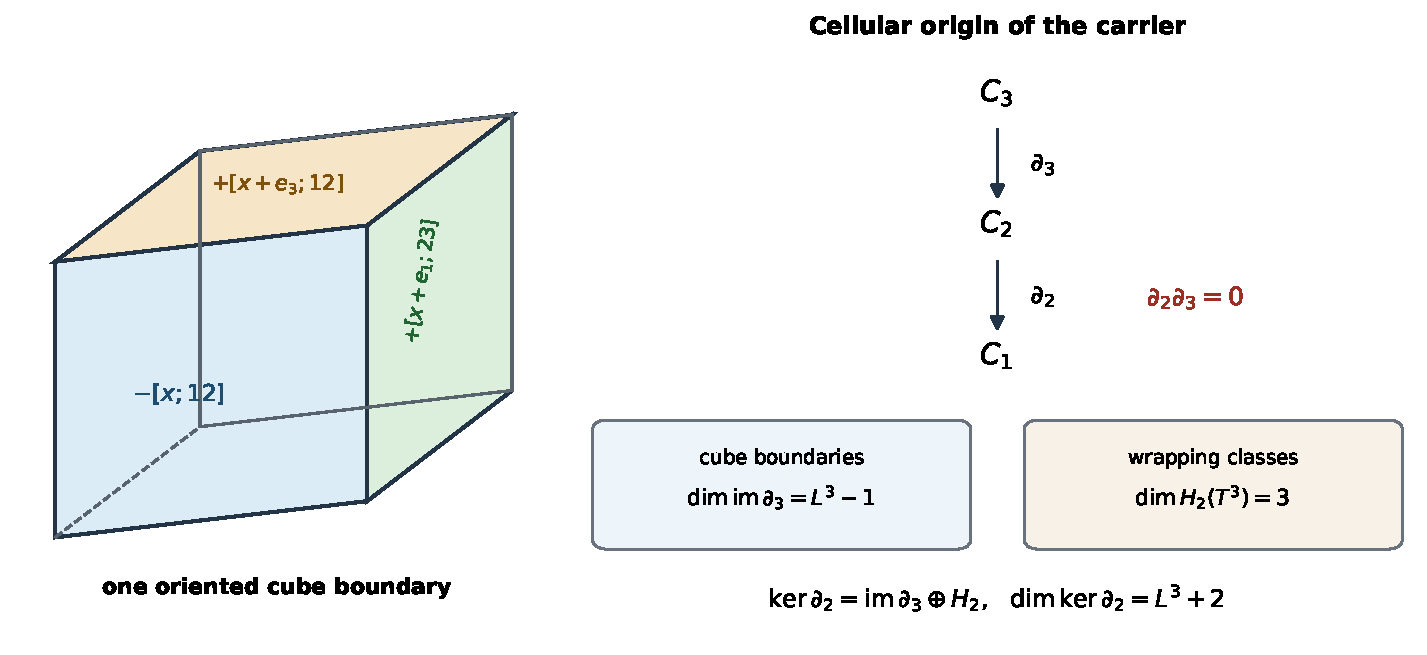
\includegraphics[width=0.97\textwidth]{figure_cellular_carrier.pdf}
\caption{The carrier is a cellular cycle space. The left panel shows three
visible terms in the outward-oriented boundary of one cube; the complete
six-face formula is given in Appendix~\ref{app:chain}. Cube boundaries span
$\operatorname{im}\partial_3$, while three noncontractible wrapping classes
complete $\ker\partial_2$ on the three-torus.}
\label{fig:cellular}
\end{figure}

The count is verified over $\mathbb{Z}$ rather than re-derived from the
formula: the complex is built from the boundary formulas of
Appendix~\ref{app:chain}; the exhibited cycles --- every elementary cube
boundary together with three wrapping sheets --- bound the kernel from below,
and rank over $\mathbb{F}_p$ bounds it from above, since rank can only drop
under reduction. The two bounds meet at $L=1,\dots,5$.
\chk{dim Z\_2 = L\^{}3 + 2 by rank, not by re-arranging the formula}
\chk{cube boundaries and three wrapping sheets SPAN Z\_2}

\begin{remark}
$L^3+2$ is the nullity of the down boundary Laplacian, not a Betti number; the
Betti contribution is the final $3$. The restriction $L\ge3$ belongs to the
twelve-neighbour Bloch adjacency, where $x+e$ and $x-e$ coincide at $L=2$. The
chain-level count has no such restriction and holds at $L=1,2$ as well.
\chk{the L\^{}3+2 count is chain-level, not the Bloch convention}
\end{remark}

The following sum rule joins Theorems~\ref{thm:fact} and~\ref{thm:carrier},
which are otherwise two unrelated statements: a $3\times3$ spectrum and an
$(L^3+2)$-dimensional space.

\begin{theorem}[Bloch--chain bridge]\label{thm:bridge}
On the periodic $L^3$ complex,
\[
  \sum_{k}\bigl(3-\operatorname{rank}B(k)\bigr)=L^3+2 ,
\]
the sum running over the $L^3$ allowed momenta, with nullity profile
$3$ at $\Gamma$ exactly once and $1$ at each of the other $L^3-1$ momenta.
\end{theorem}

\begin{proof}
$B(0)=0$ contributes $3$. For $k\neq0$ some $d_j\neq0$, and
Theorem~\ref{thm:fact} gives $\operatorname{rank}B(k)=2$, contributing $1$
each. Summing gives $3+(L^3-1)=L^3+2$.
\end{proof}
\chk{the Bloch and chain routes to the carrier agree}

\begin{remark}
Earlier editions of this paper read the agreement as a coincidence worth
checking --- ``the $3$ is the triple degeneracy of $B(0)=0$, not $b_2(T^3)$''.
That was wrong, and the correction is the better statement. Under the discrete
Fourier transform $\partial_2$ block-diagonalises and
$\ker\partial_2=\bigoplus_k\ker\partial_2(k)$; at $k\neq0$ the kernel block is
one-dimensional and is exactly $\operatorname{im}\partial_3(k)$, while
$\partial_3(0)=0$. So all of $\operatorname{im}\partial_3$ sits at nonzero
momenta and the quotient is supported entirely at $\Gamma$: the $\Gamma$ block
\emph{is} $H_2$, and the $3$ \emph{is} $b_2(T^3)$. The two routes do not agree
by accident; they are the same decomposition read in two bases.
\chk{the sheets average to harmonic representatives, and the Gamma block IS b\_2}
\end{remark}

\subsection{The wrapping sheets are cycles, not harmonic --- and their
harmonic representatives}

Theorem~\ref{thm:carrier} exhibits its three $H_2$ generators explicitly as
wrapping sheets $s_{(ij)}=\sum_{x:\,x_m=0}[x;i,j]$. These satisfy
$\partial_2 s=0$ exactly, so they are cycles and they span the quotient
$\ker\partial_2/\operatorname{im}\partial_3$. They are \emph{not} harmonic:
$\partial_3\dg s\neq0$, and
\begin{equation}
  \frac{\langle s,\;\partial_3\partial_3\dg\,s\rangle}{\|s\|^2}=2
  \qquad\text{exactly, for every }L\ge2 .
\end{equation}
\chk{FINDING: the wrapping sheets are cycles but NOT harmonic}

The distinction matters because $H_2$ is used in two senses: the quotient in
Theorem~\ref{thm:carrier}, which the sheets span, and the harmonic subspace
$\ker\partial_2\cap\ker\partial_3\dg$, which they do not lie in.

Harmonic representatives do exist, and they are one line away. Averaging a
sheet over its $L$ translates in the complementary direction,
\begin{equation}\label{eq:harm}
  h_{(ij)}=\frac1L\sum_{r=0}^{L-1}s_{(ij)}(r),
  \qquad
  \partial_2h_{(ij)}=0,\quad \partial_3\dg h_{(ij)}=0 ,
\end{equation}
gives three harmonic chains spanning
$\ker\partial_2\cap\ker\partial_3\dg$, which is exactly three-dimensional;
and $s_{(ij)}-h_{(ij)}\in\operatorname{im}\partial_3$, so a sheet and its
average are the same homology class. The averaging is the $k=0$ Fourier
projection, and what it removes is precisely the non-harmonic part measured
above. Nothing about the finding is withdrawn --- the generators
Theorem~\ref{thm:carrier} exhibits are still not harmonic --- but a real-space
statement phrased for the harmonic subspace now has representatives to point
at, and Proposition~\ref{prop:rigid} covers both, since $B\dg w=0$ holds on
all of $\ker\partial_2$.
\chk{the sheets average to harmonic representatives, and the Gamma block IS b\_2}

\section{Exact adjacent shared-link dynamics and conditional assembly}
\label{sec:second}

Two plaquettes sharing a link leave six nonshared fundamental links after the
external contractions. On the shared link the fusion channels depend on the
relative induced orientation,
\begin{equation}\label{eq:fusion}
  F\otimes\bar F=\mathbf{1}\oplus\mathrm{Adj},
  \qquad
  F\otimes F=\Lambda^2F\oplus\mathrm{Sym}^2F ,
\end{equation}
with dimensions and quadratic Casimirs
\begin{equation}\label{eq:table}
\begin{aligned}
  d_{\mathbf 1}&=1, & C_{\mathbf 1}&=0,\\
  d_{\mathrm{Adj}}&=N^2-1, & C_{\mathrm{Adj}}&=N,\\
  d_{\Lambda^2F}&=\tfrac{N(N-1)}2, & C_{\Lambda^2F}&=\tfrac{(N+1)(N-2)}N,\\
  d_{\mathrm{Sym}^2F}&=\tfrac{N(N+1)}2, & C_{\mathrm{Sym}^2F}&=\tfrac{(N-1)(N+2)}N.
\end{aligned}
\end{equation}

\begin{lemma}[The channel list is complete]\label{lem:channels}
For every $N\ge3$, a second-order process through one shared link has its
intermediate shared-link representation in
$\{\mathbf1,\mathrm{Adj},\Lambda^2F,\mathrm{Sym}^2F\}$ up to conjugation, and
in nothing else. The conjugate of a channel carries the same Casimir and hence
the same weight, which is why four labels suffice where the link-resolved
census of Section~\ref{sec:twocube} needs six.
\end{lemma}

\begin{proof}
The shared link of a one-plaquette shell state carries $F$ or $\bar F$; one
plaquette action tensors it by $F$ or $\bar F$; and \eqref{eq:fusion}, together
with the conjugate product
$\bar F\otimes\bar F=\Lambda^2\bar F\oplus\mathrm{Sym}^2\bar F$, decomposes
every case completely and multiplicity-free. There is nothing else for the link
to carry.
\end{proof}
\chk{each channel gap is C\_F + C\_R/2, and the weights sum to one}

\noindent The corollary that makes this checkable rather than merely stated is
that the weights $d_\rho/N^2$ sum to one within each orientation family, which
is arithmetic on \eqref{eq:table}: a missing channel would leave a deficit.
What Lemma~\ref{lem:channels} does \emph{not} settle is that one-shared-link
processes exhaust the second-order off-diagonal intermediates --- that is
Lemma~\ref{lem:exhaust}, and it is a statement about the process enumeration
rather than about this list.

The six nonshared half-links contribute $3\CF$ and the fused link $C_\rho/2$,
against an external one-plaquette energy $2\CF$, so the resolvent denominator
is $\CF+C_\rho/2$ exactly.
\chk{each channel gap is C\_F + C\_R/2, and the weights sum to one}

\subsection{The channel weights are a theorem}

Earlier editions assigned the channel projector squared norm $d_\rho/N^2$ by
an isotropy hypothesis, and every statement in this section rests on that
assignment. It is not a hypothesis.

\begin{theorem}[Shared-link channel weights]\label{thm:weingarten}
In the normalised two-plaquette state, the weight of the shared-link channel
$\rho$ is exactly $d_\rho/N^2$, for both orientation families and every
$N\ge3$.
\end{theorem}

\begin{proof}
Two steps. First the six nonshared links collapse. Each plaquette contributes
a product of three independent Haar links, and a product of independent Haar
matrices is Haar, so the amplitude is
$\operatorname{Tr}(AU)\operatorname{Tr}(BU^{\pm1})$ with $A,B$ independent
Haar and $U$ the shared link. Integrating $A$ and $B$ contributes
$\delta/N$ each and leaves a pure degree-$(2,2)$ moment of $U$.

Second, two such moments settle both families. In the Weingarten calculus,
whose asymptotic origin is~\cite{Weingarten1978} and whose finite-$N$ closed
forms are~\cite{CollinsSniady2006}, the order-two values are
$\mathrm{Wg}(e)=1/(N^2-1)$ and
$\mathrm{Wg}((12))=-1/(N(N^2-1))$ --- the inverse of the $S_2$ Gram matrix
$\bigl(\begin{smallmatrix}N^2&N\\N&N^2\end{smallmatrix}\bigr)$ --- the index
sums give
\begin{equation}\label{eq:moments}
  \begin{aligned}
    M_{\mathrm{direct}}&=\sum_{ijkl}\bigl\langle|U_{ij}|^2|U_{kl}|^2\bigr\rangle=N^2,\\
    M_{\mathrm{cross}}&=\sum_{ijkl}\bigl\langle U_{ij}U_{kl}\bar U_{il}\bar U_{kj}\bigr\rangle=N .
  \end{aligned}
\end{equation}
The standard formula is often written for $U(N)$. The present degree-$(2,2)$
integrands are invariant under $U\mapsto zU$, so disintegrating Haar measure
over the central $U(1)$ shows that their normalised $U(N)$ and $SU(N)$
integrals coincide. No determinant-sector term occurs at this degree for
$N\ge3$.
For the like family, $\operatorname{Tr}(AU)\operatorname{Tr}(BU)$ decomposes
into $\mathrm{Sym}^2\oplus\Lambda^2$ by symmetrising the two index pairs
jointly, and the two squared norms are
$(M_{\mathrm{direct}}\pm M_{\mathrm{cross}})/2$. Normalising,
\[
  n_{\mathrm{Sym}^2}=\frac{N+1}{2N}=\frac{d_{\mathrm{Sym}^2F}}{N^2},
  \qquad
  n_{\Lambda^2}=\frac{N-1}{2N}=\frac{d_{\Lambda^2F}}{N^2}.
\]
For the mixed family the singlet component of $U_{ij}\bar U_{lk}$ is
$\delta_{il}\delta_{jk}/N$, of squared norm $1$ against
$M_{\mathrm{direct}}=N^2$, so $n_{\mathbf 1}=1/N^2=d_{\mathbf 1}/N^2$ and
$n_{\mathrm{Adj}}=1-1/N^2=d_{\mathrm{Adj}}/N^2$.
\end{proof}
\chk{the shared-link weights are Weingarten, not an isotropy assumption}

\begin{remark}
The derivation imports nothing: the Weingarten pair is the inverse of the
$S_2$ Gram matrix and the index sums in \eqref{eq:moments} are explicit, so
the reader can check it without leaving this page. That the pair is not two
fitted constants is separately checked --- the identity-permutation value times
$N^2-1$ is $1$ identically in $N$, so the $SU(3)$ numbers are a specialisation
of a rank-generic formula. Together these make the \emph{local shared-link
coefficient} self-contained. They do not enumerate every second-order process
or prove the global torus assembly. Appendix~%
\ref{app:wg} records the index sums.
\chk{the Weingarten route is independent of the corpus}
\end{remark}

\begin{remark}[External corroboration]
The same numerator appears in the quantum-simulation literature from an
unrelated direction. Ciavarella, Burbano and Bauer~\cite{CBB2025} publish a
finite-rank plaquette matrix element
$|M_\rho|^2=\dim\rho/(\dim A\,\dim R)$; for two fundamental factors
$\dim A=\dim R=N$ and this is $d_\rho/N^2$ identically in $N$. That is
provenance for a chain already checked here, not a second derivation, and it
does not check the premise that four channels exhaust the shared-link routes.
\chk{the published dimension-ratio matrix element is this registry's weight formula}
\end{remark}

\begin{remark}[A falsified zero backend]
The organized authority corpus contains an independent exact diagnostic at
$N=3$:
\[
 \mathrm{Wg}(e)=\frac18,\qquad
 \mathrm{Wg}((12))=-\frac1{24},\qquad
 \int_{SU(3)}|U_{11}|^4\,dU=\frac16\ne0.
\]
It therefore falsifies the archived stranded-flux rule that discards this
balanced Haar sector. This is useful negative evidence for retaining the
contractions above; it is not a second derivation of $t_N$.
\end{remark}

A channel's squared projector norm and its signed contribution to the cross
matrix element are related but not identical statements, and the step between
them deserves its own displayed equation rather than a jump. For each
intermediate irrep $\rho$, with $Q_\rho$ the projector onto the
$E=3\CF+C_\rho/2$ intermediate carrying $\rho$ on the shared link,
\begin{equation}\label{eq:channelme}
  \langle p',-|VQ_\rho V|p,-\rangle
  =\eta_\rho\,s(p',e)\,s(p,e)\,\frac{d_\rho}{N^2},
  \qquad
  \eta_\rho=
  \begin{cases}
    -1,&\rho\in\{\mathbf1,\mathrm{Adj}\}\ \text{(mixed family)},\\
    +1,&\rho\in\{\Lambda^2F,\mathrm{Sym}^2F\}\ \text{(like family)},
  \end{cases}
\end{equation}
where $d_\rho/N^2$ is the Weingarten weight of
Theorem~\ref{thm:weingarten}, the incidence signs come from the oriented
boundaries, and $\eta_\rho$ is the charge-odd family sign: reversing the
induced orientation on one face interchanges the families and flips the
charge-odd combination. Inserting the reduced resolvent, whose denominator
against the external energy $2\CF$ is $\CF+C_\rho/2$ exactly,
\begin{equation}\label{eq:channelres}
  \langle p',-|VQ_\rho(E_{F,N}-H_E)^{-1}Q_\rho V|p,-\rangle
  =-\eta_\rho\,s(p',e)s(p,e)\,\frac{d_\rho/N^2}{\CF+C_\rho/2}.
\end{equation}
Summing \eqref{eq:channelres} over the four channels is the whole content of
the theorem below. With Theorem~\ref{thm:weingarten} the resolvent weight is
\begin{equation}\label{eq:w}
  w_\rho=-\frac{d_\rho/N^2}{\CF+C_\rho/2},
\end{equation}
and summing within the two orientation families,
\begin{align}
  A_N&=w_{\mathbf 1}+w_{\mathrm{Adj}}=-\frac{2N^3}{(N^2-1)(2N^2-1)},\label{eq:AN}\\
  B_N&=w_{\Lambda^2}+w_{\mathrm{Sym}^2}=-\frac{4N(N^2-2)}{(N^2-1)(4N^2-9)}.\label{eq:BN}
\end{align}
\chk{the four channel weights follow from dimension and Casimir}
\chk{A\_N and B\_N are the channel sums, not transcriptions}

\subsection{The shared-link law}

\begin{theorem}[All-rank adjacent shared-link law]\label{thm:allrank}
Let $p\ne p'$ be oriented plaquettes sharing the single link $e$. For every
integer $N\ge3$, the linked order-$u^2$ contribution through the four fusion
channels in \eqref{eq:fusion} is
\[
  \langle p',-|K^{(2)}_-|p,-\rangle
  =t_N\,s(p',e)s(p,e)
  =t_N(BB\dg)_{p'p},
\]
where $s(p,e)=\pm1$ is the cellular boundary incidence and
\[
  t_N=B_N-A_N=\frac{2N(N^2-4)}{(N^2-1)(2N^2-1)(4N^2-9)}>0 .
\]
\end{theorem}

\begin{proof}
Because distinct cubical faces share at most one link,
$(BB\dg)_{p'p}=s(p',e)s(p,e)$. Reversing the induced orientation on one face
interchanges the mixed and like fusion families. In the charge-odd
combination that reversal changes the sign, so the oriented matrix element is
the family difference $B_N-A_N$ times the incidence product. Substituting
\eqref{eq:AN}--\eqref{eq:BN} gives the displayed rational function. For
$N\ge3$ every denominator factor is positive and $N^2-4>0$.
\end{proof}
\chk{t\_N = B\_N - A\_N}\chk{t\_N > 0 for N >= 3}
\chk{two distinct torus faces share at most one link, exhaustively at L = 3 and 4}

The opening geometric ingredient of the proof is no longer prose: the
verifier enumerates every distinct face pair of the periodic complex at
$L=3$ and $L=4$ and confirms that no pair meets in more than one link. Two
faces sharing a link span at most two sites per axis, so these windows
already exhibit every local configuration and larger $L$ adds translates
only.

\begin{conditional}[Global torus assembly]\label{cor:assembly}
Assume (i) the retained-shell hypothesis of Section~\ref{sec:carrier} and
(ii) that adjacent one-shared-link routes exhaust all second-order
off-diagonal intermediates. Translation and cubic symmetry then make the
remaining diagonal contribution a scalar, and
\[
  H^{(N)}_{\mathrm{eff},-}(k,u)
  =E_{\mathrm{flat},N}(u)I+t_Nu^2B(k)B(k)\dg+O(u^3).
\]
Consequently the three bands through second order are
$E_{\mathrm{flat},N}(u)$ and
$E_{\mathrm{flat},N}(u)+t_Nu^2q(k)$ twice.
\end{conditional}

\begin{proof}
Under assumption (ii), Theorem~\ref{thm:allrank} assembles every off-diagonal
entry. Translations act transitively on faces of a fixed orientation and the
cubic group permutes the orientations, so any invariant diagonal is a multiple
of the identity. Thus the adjacency part is
$t_N(BB\dg-4I)$; absorb $-4t_N$ into the scalar and apply
Theorem~\ref{thm:fact}. The two assumptions are not consequences of the
channel calculation and are retained explicitly.
\end{proof}

Both assumptions are discharged in Section~\ref{sec:closing}
(Lemmas~\ref{lem:shell} and~\ref{lem:exhaust}), which upgrades this
corollary to Theorem~\ref{thm:assembly}; the conditional form is kept above
so the logical dependence stays legible.

Two consequences,
\begin{equation}\label{eq:tsmall}
  t_3=\frac{5}{612},\qquad
  t_N=\frac1{4N^3}-\frac1{16N^5}-\frac{77}{64N^7}-\frac{1021}{256N^9}+\cdots
\end{equation}
\chk{t\_2 = 0 and t\_3 = 5/612}\chk{large-N expansion of t\_N through 1/N\^{}9}

The expansion is governed by a closed form. Writing the planar-normalised
coefficient as $4N^3t_N$,
\begin{equation}\label{eq:planar}
  1-4N^3t_N=\frac{2N^4+31N^2-9}{(N^2-1)(2N^2-1)(4N^2-9)},
\end{equation}
an identity of rational functions, and the right side is positive and the
left strictly decreasing for every real $N\ge2$: substituting $N=M+2$ makes
every numerator coefficient of both the remainder and the derivative
nonnegative, so $4N^3t_N$ increases monotonically to $1$. At fixed canonical
coordinate $u$ the conditional bandwidth of Corollary~\ref{cor:assembly} is
$12t_Nu^2$, so the entire dispersive content of the projected sector
switches off at exactly the rate $N^{-3}$, with computable subleading
coefficient $-1/(4N^2)$: conditional on the assembly, the carrier's exact
degeneracy is approached by the \emph{whole} sector in the planar limit.
This is consistent with the general suppression of glueball mixing at large
$N$, but no 't~Hooft-coupling identification is made here: the statement is
about the coefficient in the canonical coordinate, and it is exact.
\chk{1 - 4N\^{}3 t\_N has the closed form of eq. (planar), positive for all N >= 2}
\chk{4N\^{}3 t\_N increases monotonically to 1: shifted derivative coefficients are nonnegative}

\subsection{The vacuum-mediated route}

The proof of Theorem~\ref{thm:allrank} asserts that only shared-link routes
survive. That is false in general and true here, for a reason worth stating:
it is a charge-conjugation selection rule, and omitting it is a recorded
error, not a hypothetical one.

\begin{proposition}[Vacuum-mediated route]\label{prop:vacuum}
The reduced-resolvent route
\[
 \frac{\langle p'|V|0\rangle\langle 0|V|p\rangle}{E_{F,N}-E_0}
 =\frac{\langle p'|V|0\rangle\langle 0|V|p\rangle}{E_{F,N}}
\]
is available for any
pair of plaquettes, sharing a link or not. It vanishes identically in the
charge-odd sector, because $V$ is charge-even and $|0\rangle$ is charge-even,
so $\langle0|V|p,-\rangle=0$. Consequently the charge-odd hopping
$t_N=B_N-A_N$ carries no such term, while the charge-even shared-link element
acquires $1/\CF$: the normalised charge-even matrix-element product is $2$
and $E_{F,N}=2\CF$.
\[
  \ell_N=A_N+B_N+\frac1{\CF}
  =-\frac{2N(3N^2-5)}{(N^2-1)(2N^2-1)(4N^2-9)} .
\]
\end{proposition}
\chk{ell\_N = A\_N + B\_N + 1/C\_F, the vacuum-mediated route at every rank}

\begin{remark}
At $N=3$, $A_3+B_3=-481/612$ and $1/\CF=3/4$, giving $\ell_3=-11/306$. The
first of these is exactly the value once published for the charge-even hopping
and later superseded; the correction is precisely the omitted route. Stating
the selection rule turns a one-rank erratum into an all-rank formula.

One thing this proposition does \emph{not} do is dispose of the route between
non-adjacent pairs. Taken over all pairs it would be a rank-one operator
supported at $k=0$, which is not the twelve-neighbour adjacency $\ell_N$
multiplies; which contributions survive in $K^{(2)}_-$ is settled by the linked,
vacuum-subtracted prescription of \eqref{eq:heff}, not by anything derived
here. What the check above establishes is the all-rank value $\ell_N$ of the
shared-link element, and the disposition of the non-adjacent contributions is
prescription rather than result.
\end{remark}

\subsection{Closing the two premises}
\label{sec:closing}

Both premises of Corollary~\ref{cor:assembly} --- until this edition the two
load-bearing prose hypotheses of the paper --- admit proofs. They are given
here for the first time; their combinatorial cores are machine-checked, their
single representation-theoretic input is classical and named, and a reader
should audit them with the same hostility as everything else: they are new
in this edition and have not yet survived external referees.

\begin{lemma}[Retained shell]\label{lem:shell}
Fix $N\ge3$ and $L\ge3$, in the cyclic gauge-invariant sector with trivial
electric centre flux, excluding at $L=4$ the straight winding loops as in
Section~\ref{sec:carrier}. The $E=E_{F,N}=2\CF$ eigenspace of $H_E$ is
exactly the span of the single-plaquette states, and its charge-odd part is
the span of the $|p,-\rangle$.
\end{lemma}

\begin{proof}
In the electric basis a gauge-invariant state assigns an irrep $\rho_e$ to
each link and an intertwiner to each site, with energy
$\sum_e C(\rho_e)/2$ over the nontrivially charged links. The one classical
input: for $SU(N)$ the quadratic Casimir of every nontrivial irrep satisfies
$C(\rho)\ge\CF$, with equality exactly for $F$ and $\bar F$ (the fundamental
weights $\omega_1,\omega_{N-1}$ are minuscule and $C(\lambda)
=\langle\lambda,\lambda+2\delta\rangle$ grows strictly along the dominance
order). So a state at $2\CF$ has $k\le4$ charged links.

Geometry now does the rest, with no further representation arithmetic. A
$1$-valent site is never invariant, and a $2$-valent site forces conjugate
irreps on its two links, so the charged sublattice has minimum degree $2$ at
charged sites and any junction has valence $\ge3$. With
$\sum_{\text{sites}}\deg=2k\le8$: valence-$3$ junctions come in pairs
($3j+2v=2k$ with $j$ even by parity of ends), and two $3$-valent junctions
with $k\le4$ require three disjoint paths of lengths summing to $\le4$,
hence lengths $(1,1,1)$ or $(1,1,2)$ --- both demand two distinct links
between one pair of adjacent sites, which the simple cubic torus does not
have. A $4$-valent junction with $k=4$ requires all four links to close
pairwise through $2$-valent sites, again demanding parallel links. Cycles
shorter than $4$ need care, because the odd-$L$ torus is \emph{not}
bipartite: exhaustive enumeration (machine-checked at $L=3,4,5$) shows the
only closed link sets of length $<4$ are the $3L^2$ straight winding
triangles at $L=3$. A winding triangle carries one irrep $\rho$ around a
noncontractible cycle: if $\rho$ has nonzero $N$-ality the trivial-centre-flux
sector removes it, and if zero $N$-ality then $C(\rho)\ge C_{\mathrm{Adj}}=N$
(the second classical input: the quasi-minuscule highest root minimises the
Casimir on the nonzero root lattice), so its energy $3C(\rho)/2\ge3N/2>2\CF$.
Two disjoint closed components need $\ge8$ charged links. So the charged
sublattice at $E=2\CF$ is a single $4$-cycle of $2$-valent sites: one irrep
$\rho$ runs around it (conjugated with orientation), the energy is
$2C(\rho)=2\CF$, and minimality forces $\rho\in\{F,\bar F\}$.

Finally, every $4$-cycle of the torus at $L\ge3$ is an elementary plaquette
except, exactly at $L=4$, the straight winding loops --- machine-checked by
exhaustive enumeration of all length-$4$ closed link paths at $L=3,4,5$ ---
and the winding loops are removed by the sector qualification. The
$E$-eigenspace is therefore spanned by the two orientation states of each
plaquette, and its charge-odd part by the $|p,-\rangle$.
\end{proof}
\chk{the torus graph is simple, and the only short cycles are the L = 3 winding triangles}
\chk{every 4-cycle is an elementary face, except exactly the 3L\^{}2 straight winding loops at L = 4}

\begin{lemma}[Second-order process exhaustion]\label{lem:exhaust}
For $p\ne p'$ in the charge-odd one-plaquette sector, every nonvanishing
second-order route $\langle p',-|VQ(E_{F,N}-H_E)^{-1}QV|p,-\rangle$ has its
two $V$-insertions supported on the faces $p$ and $p'$ themselves. In
particular, when $p$ and $p'$ share no link the off-diagonal element
vanishes, and when they share one link it is exhausted by the four fusion
channels of Theorem~\ref{thm:allrank}.
\end{lemma}

\begin{proof}
$V$ is a sum of single-plaquette terms, and multiplying by
$\operatorname{Tr}U_q^{\pm1}$ changes the electric content only on the four
links of $q$; the resolvent is diagonal in the electric basis and changes
none. Two insertions $q_1,q_2$ therefore leave every link outside
$\operatorname{supp}q_1\cup\operatorname{supp}q_2$ untouched, so
$p\,\triangle\,p'\subseteq\operatorname{supp}q_1\cup\operatorname{supp}q_2$.
The set $p\setminus p'$ has three links (shared-link pair) or four
(otherwise), and by the exhaustive shared-link geometry a face distinct from
$p$ contains at most one link of $p$: two insertions not supported on $p$
cover at most two of them. Hence one insertion is supported on $p$, and
symmetrically the other on $p'$; for $p\ne p'$ that pins
$\{\operatorname{supp}q_1,\operatorname{supp}q_2\}=\{p,p'\}$ exactly.

It remains to dispose of the routes this still allows beyond the fusion
channels. If $p$ and $p'$ are disjoint (sharing a vertex or nothing), both
orders factor through a local charge parity: annihilating the $p$-flux costs
$\langle0_p|(\operatorname{Tr}U_p+\operatorname{Tr}U_p\dg)|p,-\rangle=0$,
the selection rule of Proposition~\ref{prop:vacuum}, whether the intermediate
is the vacuum or the two-plaquette state $|p\rangle\otimes|p'\rangle$; and
the order that excites $p$ first leaves adjoint flux on $p$ that the
remaining insertion, supported on $p'$, cannot clear. If they share one
link, the two insertion orders are precisely the two orientation families
of Theorem~\ref{thm:allrank}, whose intermediate content on the shared link
is the four fusion channels; an insertion orientation that drives a
nonshared link into $\Lambda^2F\oplus\mathrm{Sym}^2F$ cannot be returned to
the trivial representation by the other insertion and contributes zero. The
diagonal $p=p'$ terms are unconstrained by this argument and remain the
scalar of Corollary~\ref{cor:assembly}.
\end{proof}
\chk{two distinct torus faces share at most one link, exhaustively at L = 3 and 4}

\begin{theorem}[Global torus assembly, unconditional]\label{thm:assembly}
For $N\ge3$ and $L\ge3$, in the sector of Lemma~\ref{lem:shell}, the
charge-odd effective Hamiltonian through second order is
\[
  H^{(N)}_{\mathrm{eff},-}(k,u)
  =E_{\mathrm{flat},N}(u)I+t_Nu^2B(k)B(k)\dg+O(u^3),
\]
with the three bands $E_{\mathrm{flat},N}(u)$ and
$E_{\mathrm{flat},N}(u)+t_Nu^2q(k)$ twice, and flat carrier
$\ker\partial_2$ of dimension $L^3+2$.
\end{theorem}

\begin{proof}
Lemma~\ref{lem:shell} discharges assumption (i) of
Corollary~\ref{cor:assembly} and Lemma~\ref{lem:exhaust} assumption (ii);
the corollary's own proof then runs unchanged.
\end{proof}

The status change deserves one sober sentence rather than celebration. What
was conditional is now proved relative to the standard degenerate
perturbation framework of \eqref{eq:heff}, one classical Casimir-minimality
fact, and finite combinatorics that a machine has enumerated; the charge-even
identification of Section~\ref{sec:even} remains a hypothesis, and nothing
about convergence, higher orders, or the continuum has changed.

\subsection{Finite-volume width}

Let $q_{\max}(L)$ be the largest sampled $q$ on the periodic $L^3$ grid. Then
\begin{equation}\label{eq:qmax}
  q_{\max}(L)=
  \begin{cases}
    12, & L\text{ even},\\[2pt]
    12\cos^2\!\bigl(\pi/2L\bigr), & L\text{ odd},
  \end{cases}
\end{equation}
because only at even $L$ does some $k_j$ reach $\pi$ exactly. The width of the
full retained charge-odd manifold is $W^{(-)}_{N,L}=q_{\max}(L)\,t_Nu^2+O(u^3)$,
so for even $L$, and coefficientwise as $L\to\infty$ at fixed perturbative
order, $[u^2]W^{(-)}=12t_N\sim3/N^3$.
This concerns the stiffness of the dispersive doublet, not motion of the
lowest branch, which is flat at this order.
\chk{the zone maximum of q is 12 only at even L}

The smallest nonzero incidence eigenvalue is $q_{\min}=4\sin^2(\pi/L)$,
attained by one unit of momentum in a single direction.
\chk{q\_min on the L-torus grid is 4 sin\^{}2(pi/L)}

\begin{figure}[t]
\centering
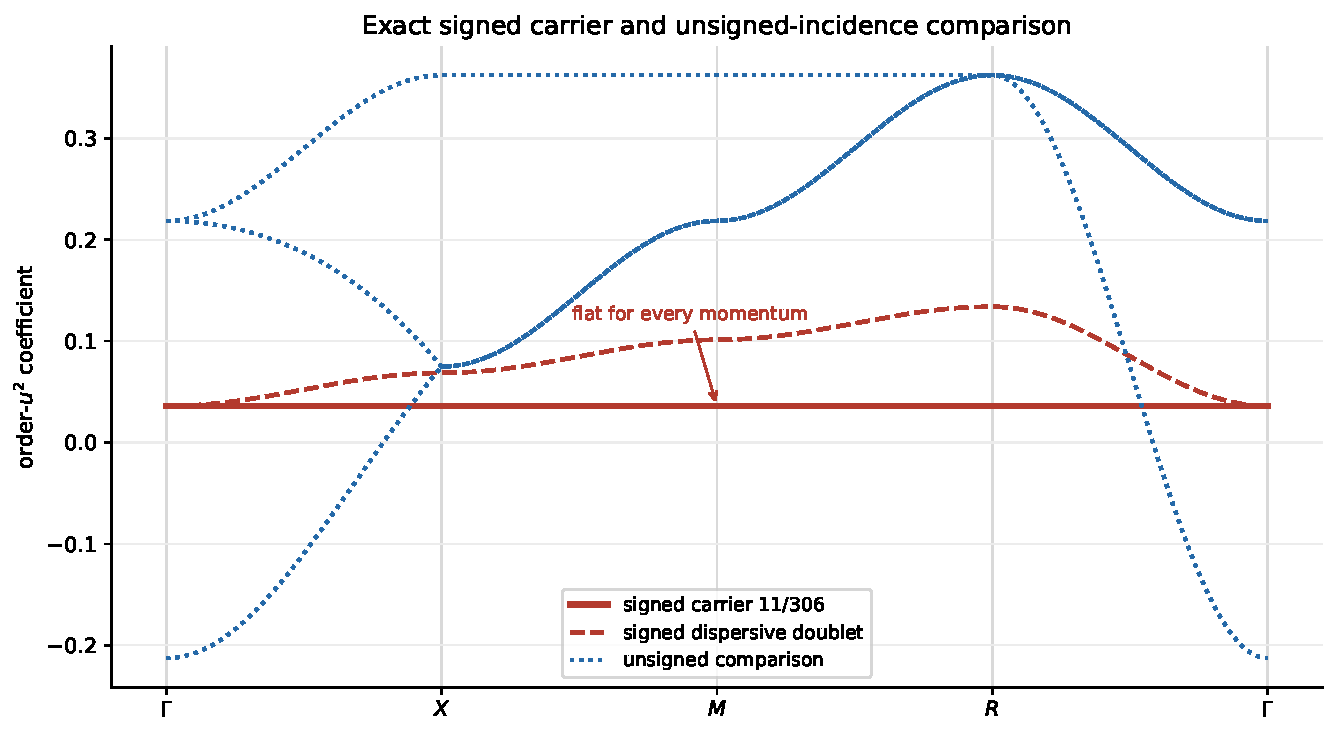
\includegraphics[width=0.94\textwidth]{figure_second_order_bands.pdf}
\caption{Order-$u^2$ coefficients along
$\Gamma$--$X$--$M$--$R$--$\Gamma$. The red carrier and dispersive doublet
are the signed incidence result; their conditional global assembly is
Corollary~\ref{cor:assembly}. The blue curves are the exact unsigned-incidence
comparison spectrum. Reading the blue curves as physical charge-even bands
requires the separate symbol hypothesis of Section~\ref{sec:even}.}
\label{fig:secondorder}
\end{figure}

\subsection{The orientation signs are essential}

Removing the orientation signs --- from the entries of \eqref{eq:B} and from
the phases, so each $e^{ik}-1$ becomes $e^{ik}+1$ --- gives an unsigned
incidence $\mathcal N(k)$. Define its comparison adjacency by
$A_+(k):=\mathcal N(k)\mathcal N(k)\dg-4I$.
Its adjacency spectra at $\Gamma$ and $R$ are $\{12,0,0\}$ and $\{-4,-4,-4\}$,
which share no eigenvalue, so no level can be momentum independent. The flat
branch is therefore not a generic consequence of three face orbitals or cubic
symmetry.

Section~\ref{sec:even} computes the unsigned comparison spectrum in closed
form. The signed span is $8-(-4)=12$, giving the charge-odd second-order width
$12t_3=5/51$ at $N=3$. The unsigned continuous-zone span is
$12-(-4)=16$. Interpreting $16|\ell_3|=88/153$ as a charge-even bandwidth is
conditional on deriving the complete linked charge-even symbol; on a finite
torus the value $-4$ is sampled only when $L$ is even.
\chk{the two band spans ARE the two incidence spectra}

\section{The second-order coefficient on a two-cube space}
\label{sec:twocube}

Everything above derives $t_N$ from a resolvent ledger indexed by the fusion
channel of one shared link. That ledger is representation theory carried out on
a single plaquette pair; it has never been tested against an operator
calculation on a space large enough for two cubes to interact. This section
reports such a test and, more importantly, states what it settles.

The construction is the open face-sharing $(3,2,2)$ prism with its eleven
oriented plaquettes, in the exact-Casimir $\mathcal B=6$ $SU(3)$ truncation, of
basis dimension $1{,}590{,}462$. The delivery reports that it reaches the
relevant sector through $794$ paths and $398$ reachable states; it does not
assemble a $1{,}590{,}462$-dimensional magnetic matrix. Its complete
charge-odd one-plaquette shell at
$E_*=8/3$ has dimension eleven --- a census result and not the plaquette count.
The full $E_*$ eigenspace has dimension $22$, split $11_{C=+}\oplus11_{C=-}$ by
tensor-derived charge conjugation, and the delivery removes all $22$ from the
pseudoinverse; because the eleven columns exhaust the odd half, that agrees
with the $Q=1_--P_-$ prescription of \eqref{eq:heff}. Writing $K_{LR}$ for the raw second-order
operator and $K_L,K_R,K_F$ for the left-cube, right-cube and shared-face
operators in their own coordinates, the connected operator is defined by the
literal M\"obius fold
\begin{equation}\label{eq:mobius}
  K_{\mathrm{conn}}=K_{LR}-J_LK_LJ_L\dg-J_RK_RJ_R\dg+J_FK_FJ_F\dg ,
\end{equation}
and the same fold applied to the geometry gives $G_{\mathrm{conn}}$. The fold
is literal in the sense that no eigenvalue or fitted scalar is subtracted: each
source operator is folded in its own coordinates and lifted. The delivery
corroborates that internally by applying the same weights history by history
over its $1{,}984$ ordered two-step histories, of which $1{,}192$ cancel at
weight zero, and the two routes agree to $4.9\times10^{-15}$.

First order settles itself. On the shell $PVP=I_{11}$, so the first-order term
is nonzero but scalar: it shifts all eleven branches equally and creates no
branch ambiguity. Its connected fold then vanishes \emph{identically}, and by
counting rather than by cancellation --- each of the eleven faces is covered
exactly once by $\{L,R\}$ once the shared face is restored by $F$, so every
M\"obius weight in \eqref{eq:mobius} applied to the identity is $1-1=0$.
Second order is therefore the leading connected term and not a correction to a
first-order one.
\chk{connected first order vanishes by inclusion-exclusion, not by cancellation of numbers}

At second order the result is
\begin{equation}\label{eq:kconn}
  K^{(2)}_{\mathrm{conn}}=\frac{5}{612}\,G_{\mathrm{conn}}+D ,
\end{equation}
with $D$ diagonal and delivered. The geometry alone fixes the \emph{splitting}
inside each block and nothing else: $G_{\mathrm{conn}}$ turns out to be four
disjoint $2\times2$ blocks plus three isolated directions
(Appendix~\ref{app:twocube}), so each pair splits by $2\times5/612=5/306$ about
its own diagonal entry. Given $D$, which Appendix~\ref{app:twocube} prints,
  the spectrum is then closed form: $0$ once, $-\tfrac{15}4$ twice,
  $-\tfrac{34}9$ four times, and $-\tfrac{129}{34}$ four times ---
exact arithmetic on entries that are themselves reconstructions, a boundary
made precise below.
The delivery reports the coefficient recovered target-blind --- supplied to no
builder, graph fit, branching rule or validator --- and reports that the payload
hashes were produced before the recorded comparison, a chronology it itself
calls record-backed and only partly auditable; the value is byte-present in the
nested $\mathcal B=4$ package that the $\mathcal B=6$ build seals as an authority object, so the
defensible statement is dependency-path nonuse and not corpus-wide absence.
This paper re-thresholds those delivered gates rather
than re-running the build, including a deliberately wrong-sign control that the
held-out scaling rejects: on a $66$-dimensional held-out word space the correct
second-order residual falls with log-log slope $2.90$ while the sign-reversed
control falls with slope $2.00$, a minimum error ratio of $325$. What all this
establishes is runtime nonuse of the comparator on the delivered dependency
path, which is not a preregistration. The finite-$u$ validations are
asymmetric: the $\mathcal B=4$ delivery includes a held-out diagonalisation of
the full $4{,}180$-dimensional charge-odd space with an $O(u^3)$ residual,
whereas the $\mathcal B=6$ check is restricted to the $66$-dimensional
$P+Q_1$ star.
\chk{the connected two-cube geometry has exactly four cross-cell pairs, each -1}
\chk{the B=6 connected kernel is (5/612) G\_conn + diag, with the certified spectrum}
\chk{the certificate's own gates pass, target-blind, with the wrong-sign control rejected}

Resolving \eqref{eq:kconn} by the irreducible representation the shared link
actually carries in the ranked intermediate state gives six coefficients rather
than four, because a link distinguishes $\rho$ from $\bar\rho$:
\begin{equation}\label{eq:census}
\begin{array}{c|cccccc}
 \rho & \mathbf1 & \mathbf3 & \bar{\mathbf3} & \mathbf6 & \bar{\mathbf6} & \mathbf8\\
 \hline
 c_\rho & \tfrac1{12} & -\tfrac1{12} & -\tfrac1{12}
        & -\tfrac19 & -\tfrac19 & \tfrac{16}{51}
\end{array}
\end{equation}
\chk{the B=6 six-channel census sums to the registry's own t\_3 = 5/612}

That these six sum to $5/612$ is weak evidence: six rationals reach one target
in many ways, and a fitted set would pass it. The statement worth making is
stronger, and it is what makes this more than a coincidence of one sum. First,
though, the boundary.

The six coefficients of \eqref{eq:census} are not symbolic: the delivery
stores them as rational reconstructions of pinned finite-precision
Clebsch--Gordan contractions, with a maximum reconstruction residual of
$2.2\times10^{-15}$ per channel --- $2.1\times10^{-14}$ across the delivery's
reconstructed matrices as a whole --- and its own certificate declaring
\texttt{symbolic\_exact\_local\_amplitudes: false}. What follows is therefore
reported, conditional on those six numbers, and not a symbolic identity in the
sense of Theorem~\ref{thm:weingarten}.

\begin{reported}[The census is the Weingarten ledger]\label{rep:census}
At $N=3$ the six reconstructed link-irrep coefficients of \eqref{eq:census}
are the four fusion-channel weights \eqref{eq:w} individually:
\[
  c_{\mathbf 1}=-w_{\mathbf 1},\qquad
  c_{\mathbf 8}=-w_{\mathrm{Adj}},
\]
\[
  c_{\mathbf 3}=c_{\bar{\mathbf 3}}=\tfrac12 w_{\Lambda^2F},\qquad
  c_{\mathbf 6}=c_{\bar{\mathbf 6}}=\tfrac12 w_{\mathrm{Sym}^2F}.
\]
\end{reported}

\noindent Substituting \eqref{eq:table} into \eqref{eq:w} at $N=3$ gives
$w_{\mathbf 1}=-1/12$, $w_{\mathrm{Adj}}=-16/51$, $w_{\Lambda^2F}=-1/6$ and
$w_{\mathrm{Sym}^2F}=-2/9$; comparison with \eqref{eq:census} is then
arithmetic. Six reconstructed rationals landing on four predicted ones, with
the two coincidences the correspondence requires, is a strong consistency
statement and not a proof that the underlying contraction is exact.
\chk{the B=6 six-channel census IS the Weingarten four-channel ledger, channel by channel}

One further feature of the census is worth separating out, because it is the
paper's central architecture measured rather than assumed. The six
link-resolved matrices are not merely six numbers that sum correctly: each is
\emph{separately} proportional to the same incidence Gram. The eleven oriented
plaquettes of the prism have exactly $56$ ordered adjacent pairs, each sharing
one link with signed overlap $\pm1$; the delivery reports a constant
channel-to-geometry ratio on all $56$ of them, for every one of the six
channels, with worst residual $2.2\times10^{-15}$. Colour dynamics fixes a
number per channel and the cellular boundary operator fixes the matrix; if the
two mixed, the ratio would be constant for the total and not for the parts.
\chk{every shared-link channel is separately proportional to the geometry, on all 56 pairs}

The correspondence is scoped to what the Casimir closure exhausts: adjacent,
one-action, shared-link intermediates at order $u^2$. Same-face diagonal
routes, on-site terms and higher-action intermediates lie outside it --- the
$\mathcal B=6$ scalar below is exactly a place where one of them is missing --- and so
does any untruncated-Hilbert-space statement.

It is scoped in one further way, which matters more. The two-cube build draws
its local Wilson amplitudes from the same hash-pinned upstream
Clebsch--Gordan archive as the single-cube reconstructions of the next
subsection, and the squared amplitudes that archive produces are the published
$d_\rho/N^2$~\cite{CBB2025} --- the numerator of \eqref{eq:w}. The census
therefore does not confirm the weights from an independent source: it tests the
\emph{assembly} that carries them, which is the reachable-channel list, the
resolvent denominators, the operator-level fold, the even split between
conjugates, and the geometry that survives each channel separately. That is the
statement worth making, and it is a different statement from confirmation.

Two features of the correspondence carry the content. The mixed family enters
negated because $t_N=B_N-A_N$, which is the same relative sign the incidence
orientation carries. And each like-family \emph{fusion} weight is split evenly
between the irrep and its conjugate --- the two orientations of the shared link
weighted equally --- which the delivery resolves on the two-cube space rather
than assuming. It is not measured \emph{here}: what this repository checks is
the identity the six delivered numbers satisfy.

\begin{conjecture}[All-rank even split]\label{conj:split}
For every $N\ge3$ each like-family fusion weight splits evenly between an
irrep and its conjugate in the link-resolved census.
\end{conjecture}

\noindent This is a conjecture and nothing here promotes it. Falsifying it
means a link-resolved census at some $N\ge4$ in a truncation that still
retains every adjacent shared-link channel; at $N=4$ the endpoint budgets make
that $\mathcal B\ge33/4$, and no such construction has been run.

\subsection{One truncation, two constructions}

The two-cube space also isolates why a cutoff can reverse the sign of $t_3$.
An adjacent shared-link channel $\rho$ is reachable only if the endpoint
Casimir budget $C_2(\rho)+2C_2(\mathbf 3)$ fits inside the truncation, meaning
$C_2(\rho)+2C_2(\mathbf 3)\le\mathcal B$: the sextet needs exactly $6$ and the
adjoint $17/3$, so both survive $\mathcal B=6$ and neither survives
$\mathcal B=4$. The weak inequality is not a convenience. Both retentions this
section uses are decided by an \emph{equality}: $\Lambda^2F=\bar{\mathbf 3}$ has
budget exactly $4$ and so sits exactly on the $\mathcal B=4$ cutoff, and the
sextet sits exactly on the $\mathcal B=6$ one. Under a strict rule
$\mathcal B=4$ would reach $\{\mathbf 1\}$ alone and $\mathcal B=6$ would lose
the sextet, contradicting both delivered censuses --- so the deliveries are what
fix the convention, which is also why the budget arithmetic is not an
independent confirmation of either census.
\chk{B=6 retains every adjacent shared-link channel; B=4 provably cannot}
\chk{the retention rule is C2(rho) + 2 C2(3) <= B, and both retentions it decides are equalities}

\begin{corollary}[What a link cutoff drops]\label{cor:cutoff}
Retaining only the singlet and $\Lambda^2F$ routes projects the second-order
hopping to
\[
  w_{\Lambda^2F}-w_{\mathbf 1}=-\tfrac1{12},
\]
opposite in sign to $t_3$ and $10.2$ times larger in magnitude. What is
dropped is
\[
  w_{\mathrm{Sym}^2F}-w_{\mathrm{Adj}}=\tfrac{14}{153},
\]
and $-\tfrac1{12}+\tfrac{14}{153}=\tfrac5{612}=t_3$. This is arithmetic on
\eqref{eq:w} alone.
\end{corollary}

\noindent The published $p+q\le1$ link cutoff retains exactly those two
routes --- a per-link restriction, where $\mathcal B=4$ is a total endpoint
budget, so the two schemes agree on the retained channels at this order and are
not the same rule --- so $-1/12$ is its projected adjacent hopping and
$14/153$ is the adjacent-hopping correction that completes it --- not
$5/612$, which would double-count what it already carries. On the two-cube
space the first of those two numbers is delivered rather than inferred: a
separately sealed $\mathcal B=4$ run on the identical geometry gives
$K^{(2),\,\mathcal B=4}_{\mathrm{conn}}=-\tfrac1{12}G_{\mathrm{conn}}+D_{\mathcal B=4}$
outright, and the Casimir budgets of the previous paragraph say without
reference to any census that $\mathcal B=4$ can reach only
$\{\mathbf1,\mathbf3,\bar{\mathbf3}\}$. Conditional on \eqref{eq:census}, the
same split of the census reproduces it,
$c_{\mathbf 1}+c_{\mathbf 3}+c_{\bar{\mathbf 3}}=-1/12$, and gives the omitted
half as $c_{\mathbf 6}+c_{\bar{\mathbf 6}}+c_{\mathbf 8}=14/153$.
\chk{the B=6 six-channel census IS the Weingarten four-channel ledger, channel by channel}
\chk{FINDING: the T1 link cutoff reverses the sign of t\_3, and 14/153 is what it omits}

\begin{remark}
Two single-cube reconstructions bracket the same statement. A full $\mathcal B=4$ open
cube assembled from the pinned \texttt{ymcirc} $d=3$, $\mathcal B=4$ plaquette data
~\cite{Balaji2026,ymcirc2026} reproduces $-1/12$ and the truncated shell ordering to
$4.3\times10^{-11}$; a $\mathcal B=6$ cube reproduces $+5/612$ and the inverse ordering
to $8.4\times10^{-15}$. Both locate the missing weight at the same $14/153$.

Neither is an independent replication. Both read tabulated plaquette matrix
elements of the same lineage --- and the two-cube build draws its
Clebsch--Gordan amplitudes from the same hash-pinned \texttt{pyclebsch} archive
as the $\mathcal B=6$ cube, so that agreement is a cross-check of assembly and not of
the amplitudes. The published closed form~\cite{CBB2025} is
$d_\rho/N^2$ --- the very numerator of \eqref{eq:w}. This is a cross-check of
assembly, not a third confirmation of $t_3$; the exact rational identity is
Corollary~\ref{cor:cutoff}, which needs no tolerance. The $p+q\le1$
nomenclature and the finite-rank matrix element are both from~\cite{CBB2025},
and single-cube $SU(N)$ diagonalisation in this style goes back
to~\cite{CM2003}.

The correction to the adjacent-hopping coefficient of a published $T_1$
Hamiltonian is therefore $14/153$ and not $5/612$, which would double-count
the two routes $T_1$ already carries. One coincidence of value is worth naming:
$-1/12$ is also the singlet weight $w_{\mathbf 1}$, and the cutoff value is a
\emph{difference} of two weights, not a weight.
\chk{FINDING: a full T1 = B = 4 cube Hamiltonian reproduces -1/12 and the reversed shell}
\chk{FINDING: the B = 6 cube flips the sign back to +5/612, closing the decisive test}
\end{remark}

The $\mathcal B=6$ cube is channel-complete for the hopping and \emph{not} for the
scalar: its scalar is $39/68$ against the bridge's $11/34$, differing by
exactly $1/4$, the local same-face sextet route, which first enters at cutoff
$20/3$ --- integer label $\mathcal B=7$, so any cutoff above $20/3$ already carries it.
\chk{the B = 6 scalar misses the bridge's by exactly the same-face sextet route}

\subsection{What the cutoff moves, and where}

The connected diagonal $D$ is eleven numbers in both deliveries and is treated
as a remainder in both. It is not eleven numbers. The open prism has a symmetry
group --- the cell exchange $x\mapsto2-x$, the two transverse reflections and
the $y\leftrightarrow z$ swap, of order $16$ --- and $D$ is constant on its
orbits, which are $8+2+1$: the eight side faces, the two end caps, the shared
face.

\begin{proposition}[Where the truncation lives]\label{prop:orbit}
The eight-element orbit is exactly the support of the four cross-cell pairs,
and it is the only orbit whose diagonal value differs between the two
truncations: the end caps carry $-15/4$ and the shared face $0$ at both
$\mathcal B=4$ and $\mathcal B=6$, while the side value moves from $-7/4$ to
$-2317/612$. Together with
the four cross-cell blocks carrying the whole off-diagonal change, the entire
$\mathcal B=4\to\mathcal B=6$ difference is confined to the faces that carry connected transport.
\end{proposition}
\chk{the connected diagonal is orbit-constant, and only the transporting orbit moves}

This also says what the nonuniform $D$ is. Where the faces of a complex form a
\emph{single} orbit --- the closed cube of the next subsection, or the periodic
torus under Corollary~\ref{cor:assembly} --- orbit-constancy forces the diagonal to
be scalar, and the operator is exactly $\alpha I+tG$. The prism has three
orbits because it has a boundary. $D$ is the open boundary showing up in the
diagonal, not a failure of the incidence form.

\subsection{The one-cube shell, and why its flat level cannot move}

Those two single-cube reconstructions are usually read as numerical
cross-checks. They are more than that, because the object they diagonalise is
the same chain complex. The six faces of a cube are a closed surface, so in the
outward orientation $\ker\partial_2$ is one-dimensional and spanned by the sum
of all six --- the fundamental class, $b_2(S^2)=1$. That is
Theorem~\ref{thm:carrier} on a complex with no three-cells, where the $L^3-1$
boundaries are absent and only the class survives.

\begin{proposition}[One-cube shell]\label{prop:cube}
On the closed cube surface $G=\partial_2^{\mathsf T}\partial_2$ commutes with
all $24$ proper rotations. The combinations $b_{+i}-b_{-i}$ carry the defining
vector representation and the combinations $b_{+i}+b_{-i}$ the permutation
representation of the three unordered axes, so with the charge-odd inversion
$Pb_{+i}=-b_{-i}$ the shell is
\[
  A_1^{--}\oplus T_1^{+-}\oplus E^{--},
\]
with $G$-eigenvalues $0$, $4$, $6$ and multiplicities $1$, $3$, $2$.
Consequently $\alpha I+tG$ has levels $\alpha$, $\alpha+4t$, $\alpha+6t$.
\end{proposition}

\begin{proof}
The rotations permute the six outward faces, and $G$ is built from the boundary
map, so it commutes with the permutation action. On the antisymmetric
combinations that action is the defining representation by inspection --- $b_{+i}-b_{-i}$
transforms as $e_i$ --- and on the symmetric combinations it is the
permutation representation of $\{\pm e_i\}$, which is $A_1\oplus E$. Under
$Pb_{+i}=-b_{-i}$ the antisymmetric sector is parity even and the symmetric one
parity odd. In these sectors $G$ is $4I$ and $4I-2(J-I)$ respectively, of
spectra $\{4,4,4\}$ and $\{0,6,6\}$; since the three isotypic components have
distinct dimensions the eigenvalues attach to them uniquely.
\end{proof}
\chk{the one-cube shell is A1 + T1 + E, and its flat level is the S\^{}2 fundamental class}

Three things follow. The cubic labels are derived here rather than assigned:
both deliveries assert them and neither builds the symmetry matrices. The
$A_1^{--}$ level is Proposition~\ref{prop:rigid}'s mechanism on a second
complex --- $Gw=0$ there, so that level sits at $\alpha$ for every $t$, and no truncation, no
channel and no coefficient in dispute anywhere in this paper can move it. And
the reversal the two runs report is therefore a statement about the sign of one
number rather than about the shell as a whole: at $\mathcal B=6$ the levels are
$\{39/68,\,371/612,\,127/204\}$ and at $\mathcal B=4$ $\{37/12,\,11/4,\,31/12\}$, in
the opposite order, with $A_1^{--}$ in each case sitting exactly at the scalar.
The relative shell $\{0,4t,6t\}$ is $\{0,\,5/153,\,5/102\}$ at $\mathcal B=6$.

The finite-volume fingerprint of the 28 August finite-$N$ bridge certificate
--- a different release, and named here because a reader tracing it to the
two-cube one would find nothing --- is worth recording
because its most discriminating multiplicity is not a feature of the
truncation: on the periodic $3^3$ torus the incidence eigenvalues $0,3,6,9$
have multiplicities $29,12,24,16$, respectively, and $29=L^3+2$ is
Theorem~\ref{thm:carrier}.
\chk{the certificate's finite-volume fingerprints, and 29 = L\^{}3 + 2 is the Lean cycle count}

\begin{remark}[Scope]
Everything in this section is second order in $u$, finite volume, strong
coupling, one sector. It bears on $t_N$ and decides nothing about the
fourth-order coefficient of Section~\ref{sec:fourth}. The
$\mathcal B=6$ two-cube construction was not re-run here: its arithmetic is
audited against geometry rebuilt independently, and its diagonal $D$ is
$B$-truncated and not proved cutoff-stable. The held-out finite-$u$ validation
that rejects the wrong-sign control is a $66$-dimensional $P+Q_1$ word space
with the $Q_1$--$Q_1$ magnetic block set to zero, not the full Hamiltonian, and
no radius-three stability claim was executed. The two branches are not equally
covered: at $\mathcal B=4$ the delivery reports a direct diagonalisation of the complete
$4{,}180$-dimensional charge-odd block at four small couplings, two of them
held out, with the residual after $E_*+u+u^2\operatorname{eig}K_2$ scaling as
$u^3$; at $\mathcal B=6$ no such diagonalisation exists and the $66$-dimensional star
stands in for it. That $\mathcal B=4$ report carries no check here --- its certificate
did not travel --- and is recorded as the delivery's rather than as this
paper's. No external group has reproduced the release.
\end{remark}

\subsection{A cutoff-free radius-two witness at finite coupling}
\label{sec:radius2}

A later sealed delivery (29 August 2026) assembles the charge-odd and
charge-even $SU(3)$ two-cube Ritz operators with no Casimir cutoff at all:
the electric seed $P$ (eleven charge-odd faces), the complete one-action
frontier $Q_1$, and the exact-energy-factorized two-action frontier $Q_2$,
with cumulative odd dimensions $11$, $77$, $773$. Three nested operators are
diagonalised at each coupling --- $K_1$ on $P+Q_1$; $K_2^{\ast}$, which zeroes
exactly the $Q_2$--$V$--$Q_2$ block; and the full $K_2$ --- and every
finite-coupling Cauchy interlacing inequality between them is checked, with
recorded violation exactly $0$. All quoted quantities are invariant under
diagonal basis rephasing, which is why no signed hopping entry is read as an
observable there. The delivery is finite-precision throughout; everything in
this subsection is reported at stated tolerances, never promoted.

\begin{reported}[The rational sub-block of the cutoff-free second-order
spectrum]\label{rep:radius2}
Six of the eleven eigenvalues of the sealed cutoff-free second-order block
$C_2=BR_1B\dg$ on the odd seed are rationals to within $10^{-12}$
(the worst residual is $5\times10^{-14}$, about $30$ ulps):
\[
  -\tfrac{2429}{306}\ (\times2),\qquad
  -\tfrac{404}{51}\ (\times3),\qquad
  -\tfrac{2419}{306}\ (\times1),
\]
and the outer levels straddle the central triple by exactly
\[
  \tfrac{2429}{306}-\tfrac{404}{51}
  =\tfrac{404}{51}-\tfrac{2419}{306}
  =\tfrac{5}{306}=2t_3 .
\]
The remaining five eigenvalues are not rational at this precision.
\end{reported}

The point is what this operator was \emph{not} told. The census of
Reported result~\ref{rep:census} recovered the shared-link channel
coefficients from a build that retained those channels; here the sealed
radius-two operator retains every second-order route the two-action frontier
supports, makes no shared-link truncation, and the shared-link coefficient
$t_3=5/612$ of Theorem~\ref{thm:allrank} appears anyway --- as the exact
splitting scale of a rational sub-block, embedded in a spectrum whose other
levels are algebraic. A structural identification of that sub-block (which
face combinations carry it, and why the central level is threefold) is not
derived here and is recorded as a lead, not a claim; the open two-cube
cluster has face-inequivalent environments, so a non-scalar diagonal is
expected and no contradiction with Corollary~\ref{cor:assembly}, which is a
torus statement, arises.
\chk{the sealed rational sub-block straddle is exactly 2 t\_3 = 5/306}
\chk{six sealed eigenvalues match the three rationals to 1e-12, by a stdlib Jacobi diagonalisation}

The same delivery reports direct nested-difference coefficients at fourth
and fifth order --- for the matched odd--even gap,
$C_4^{\mathrm{gap}}=-0.8272230$ and $C_5^{\mathrm{gap}}=+4.1838863$ --- each
agreeing with an independent weak-coupling Hellmann--Feynman intercept to
better than $3\times10^{-6}$. These are increments between the nested
truncations, in the delivery's own coupling convention, and are not asserted
to be complete fourth- or fifth-order coefficients of the unablated sector
Hamiltonian; no convergence claim accompanies them.
\chk{direct C4/C5 matched-gap coefficients agree with their weak-grid intercepts to 5e-6}

One further feature bears on Section~\ref{sec:fourth}. The delivery's
fifth-order object on the eleven-dimensional seed is recorded as a
\emph{matrix}: its traceless part is nonzero, with
$\operatorname{tr}(\mathrm{shape}^2)=0.359$ and eleven recorded shape
eigenvalues. It is therefore the first delivered instrument in this corpus
whose output is not a $\Gamma$-point scalar. That observation is about the
instrument class only: the two-cube cluster carries no off-axis momentum,
and nothing here weakens Theorem~\ref{thm:obstruction} or bears on the value
of $C_{\mathrm{shp}}$.
\chk{the fifth-order seed shape is traceless with nonzero trace-square: the instrument emits more than a scalar}

\section{The unsigned-incidence comparison operator}
\label{sec:even}

The unsigned incidence $\mathcal N(k)$ of Section~\ref{sec:second} defines an
exact algebraic comparison operator
$G_+(k)=\mathcal N(k)\mathcal N(k)\dg$. Its identification with the complete
linked charge-even effective Hamiltonian is an additional hypothesis, not a
result of the shared-link calculation: Proposition~\ref{prop:vacuum} exposes
an all-pairs vacuum route whose cancellation or linked-cluster reorganisation
has not been derived. With that boundary explicit, write
\[
  \hat a_m=2+2\cos k_m=|1+e^{ik_m}|^2,\qquad p=\sum_m \hat a_m .
\]
The hat is not decoration: $\hat a_m$ is the \emph{complement} of the
$a_m=4\sin^2(k_m/2)$ used in the charge-odd shape basis \eqref{eq:shapes}
below,
$\hat a_m+a_m=4$, and that complementarity is the sum rule below.

\begin{theorem}[Unsigned-incidence Bloch cubic]\label{thm:evencubic}
$p+q=12$ pointwise, and the characteristic polynomial of
$\mathcal N\mathcal N\dg$ is
\[
  \mu^3-2p\,\mu^2+p^2\mu-4\hat a_1\hat a_2\hat a_3
  \;=\;\mu(\mu-p)^2-4\hat a_1\hat a_2\hat a_3 ,
\]
with the unsigned comparison-adjacency eigenvalues $\lambda=\mu-4$. The signed
counterpart of the same computation is $\mu(\mu-q)^2$.
\end{theorem}
\chk{the unsigned-incidence characteristic polynomial is mu(mu - p)\^{}2 = 4 a\_1 a\_2 a\_3}
\chk{p + q = 12: one zone function runs both sectors}

The algebraic closed form is complete rather than merely consistent at sampled momenta:
the characteristic polynomial of the $81\times81$ and $192\times192$ finite
plaquette adjacencies factorises coefficient for coefficient over $\mathbb Z$
into this cubic over the momentum grid.
\chk{the Bloch cubic IS the finite L = 3 and L = 4 plaquette spectrum, exactly}

\begin{proposition}[Range and attainment]\label{prop:evenrange}
$\lambda\in[-4,12]$ exactly. The top $\lambda=12$ is attained only at $\Gamma$
($\hat a_1=\hat a_2=\hat a_3=4$). The bottom $\lambda=-4$ is attained on the
whole of the three planes $k_j=\pi$, where the constant term vanishes, and only
at $R$ is it a triple root.
\end{proposition}

\begin{proof}
Write $f(\mu)=\mu(\mu-p)^2-4\hat a_1\hat a_2\hat a_3$. Then
$f(0)=-4\hat a_1\hat a_2\hat a_3\le0$ and $\mu(\mu-p)^2<0$ for $\mu<0$, so no
root lies below $0$; and $f'(\mu)=(3\mu-p)(\mu-p)>0$ for $\mu>p$, with
$\hat a_1\hat a_2\hat a_3\le(p/3)^3$ by AM--GM and
\[
 f(16)\ge16(16-p)^2-\frac{4p^3}{27}
 =\frac4{27}(12-p)(48-p)^2\ge0.
\]
Hence $\mu\in[0,16]$ and
$\lambda=\mu-4\in[-4,12]$. Equality at the top forces $p=12$ and
$\hat a_1\hat a_2\hat a_3=64$, which is $\Gamma$. Equality at the bottom is
$f(0)=0$, i.e. $\hat a_1\hat a_2\hat a_3=0$, i.e. some $k_j=\pi$; there
$f(\mu)=\mu(\mu-p)^2$ and the root $\mu=0$ is simple unless $p=0$, which is
$R$ alone.
\end{proof}
\chk{the C-even range [-4, 12] is exact; the top only at Gamma, the floor on three planes}
\chk{the C-even band touches its floor exactly on the three planes k\_j = pi}

\begin{remark}
A flat unsigned-comparison branch would need $f(\mu_0)=0$ identically in $k$,
which the constant term already forbids. Its minimum is attained on three
measure-zero planes, against the signed operator's flat band. This contrast is
an exact statement about two incidence constructions, not by itself a
derivation of two physical charge sectors.
\chk{the C-even band touches its floor exactly on the three planes k\_j = pi}
\chk{the C-even spectra at the four high-symmetry momenta}
\end{remark}

\subsection{Conditional charge-even assembly}

The shared-link coefficient at $r=2$ is all-rank and analytic. Turning it into
a charge-even band structure assumes the symbol identification stated above;
the displayed second-order scalar additionally uses the supplied
$SU(3)$ leakage/tower identification. The $r=3$ values ---
$t_{3,+}=-6335/249696$ and everything computed from it --- come from the same
supplied domino ledger as Section~\ref{sec:su3}, and are conditional on it in
the same way.

Conditional on that identification, the scalar ledger is not a list of
separate facts. Writing $\lambda$ for the
adjacency eigenvalue and $\mathrm{tower}_{r,s}$ for the within-plaquette term
in canonical $u$,
\begin{equation}\label{eq:assembly}
  E_s(\lambda,r)=\mathrm{tower}_{r,s}+12\,\mathrm{leak}_{r,s}+\lambda\,t_{r,s},
\end{equation}
with $\lambda\in\{-4,8\}$ in the signed charge-odd sector (carrier and dispersive
top), $\lambda\in\{12,-4\}$ in the unsigned comparison, and $\lambda=0$
returning the on-site diagonals. This reproduces every registered diagonal
and band value --- nine of them --- across both sectors and both orders. The
tower term is the certified coupling conversion $4\Delta_\pm(3u/2)$, where at
$N=3$ the within-plaquette one-plaquette series of the two sectors are
\begin{equation}\label{eq:bridge}
\begin{aligned}
  \Delta_-(x)&=\tfrac23+\tfrac x6+\tfrac1{18}x^2+\tfrac7{432}x^3,\\
  \Delta_+(x)&=\tfrac23-\tfrac x6+\tfrac{13}{180}x^2+\tfrac{101}{2700}x^3,
\end{aligned}
\qquad x=\frac{\beta_3}4=\frac32\,u ,
\end{equation}
in the corpus's own printed coefficients; so \eqref{eq:assembly} takes no
unregistered input. The letter $\Delta$ is reused elsewhere with other
subscripts --- the fourth-order checkpoint differences, the coefficient gap
$\Delta_C$ --- and only the sector subscript $\pm$ means this series. The twelve is a count on this
lattice, not a citation: the plaquette graph is $12$-regular and two distinct
faces share at most one link. The two towers are different objects and both
are needed: the charge-odd one contributes
$8/3+u+u^2/2+7u^3/32$ and the charge-even one $8/3-u+(13/20)u^2+(101/200)u^3$,
each of them $4\Delta_\pm(3u/2)$ on its own sector's series, so
$\mathrm{tower}_{2,-}=1/2$ against $\mathrm{tower}_{2,+}=13/20$ and
$\mathrm{tower}_{3,-}=7/32$ against $\mathrm{tower}_{3,+}=101/200$.
\chk{one assembly formula gives every registered band value}
\chk{one assembly formula gives every C-even value at both orders}
\chk{the plaquette graph is 12-regular and two faces share at most one link}

Because the supplied ledger has $\mathrm{leak}_{r,+}=t_{r,+}$ at both computed
orders, the conditional charge-even assembly collapses to
$\mathrm{tower}_{r,+}+(12+\lambda)\,t_{r,+}$, a one-parameter family in the
charge-even tower. That
equality is verified and unexplained. The order-three separation is between the
charge-odd leakage and the charge-\emph{even} hopping --- not, as an earlier
edition printed, between the charge-odd leakage and the charge-odd hopping,
which were never equal: $\mathrm{leak}_{2,-}=t_{2,+}=-11/306$ against
$t_{2,-}=5/612$ at second order, and $\mathrm{leak}_{3,-}=-12331/249696$ against
$t_{3,+}=-6335/249696$ at third. It is recorded as a unifying candidate with a
falsifier --- an order at which the two are computed independently and differ
--- not as a mechanism.
\chk{both declared coincidences, checked: one is ell\_N at all ranks, the other is bare}

\subsection{Where the rest frame is not blind}

\begin{conditional}[Charge-even $\Gamma$ splitting]\label{prop:evengamma}
If the unsigned symbol is the complete linked charge-even symbol, then at
$\Gamma$ its comparison spectrum is $\{12,0,0\}$, so the $A_1^{++}$ level
and the $E^{++}$ doublet are distinct, and
\[
  E(A_1^{++})-E(E^{++})=12\,t_{r,+}
\]
exactly: $-22/51$ at $r=2$ and $-6335/20808$ at $r=3$.
\end{conditional}
\chk{the C-even Gamma point pins t\_+, exactly where no C-odd Gamma datum can}

This is the structural counterpart of the charge-odd blindness recorded in
Section~\ref{sec:su3}. The signed spectrum at $\Gamma$ is $\{-4,-4,-4\}$, one
level, so no charge-odd rest-frame series can see the hopping; the unsigned
comparison spectrum has two levels, so the charge-even rest frame could fix
the coefficient under the symbol hypothesis. Neither half needs the incidence
ansatz, and stating them through it understates both. At $\Gamma$ the little
group is the full cubic point group, so the $3\times3$ block commutes with its
action at every order in $u$ and whether or not the correction factors through
links; Schur then decides the two sectors, and decides them differently. The
charge-odd state is the \emph{oriented} $2$-cell $e_i\wedge e_j$, on which a
proper rotation acts by its exterior square, which is the rotation itself under
Hodge duality --- the defining rep $T_1$, irreducible, commutant dimension one,
so the block is a scalar. Charge conjugation drops the orientation, so the
comparison state is the \emph{unoriented} plane and the action is the
permutation of the three axes, $A_1\oplus E$, commutant dimension two. The two
commutant dimensions are exactly the two level counts, and this half of the
statement carries no symbol hypothesis at all.
\chk{Schur alone fixes both Gamma blocks: the C-odd triple is irreducible, the C-even one is not}

The $A_1^{++}$
branch is isotropic at leading order without assuming it, with curvature
$\tfrac43|t_{r,+}|$ in all three directions --- $22/459$ at second order and
$6335/187272$ at third.
\chk{the C-even curvature is (4/3)|t\_+| at both orders, and isotropic}

On a finite $L^3$ grid the conditional charge-even width is
\[
 W^{(+)}_{r,L}=|t_{r,+}|\,[12-\lambda_{\min}^{(+)}(L)],
 \qquad \lambda_{\min}^{(+)}(L)=-4\ \Longleftrightarrow\ L\ \text{is even}.
\]
Thus it equals $16|t_{r,+}|$ for even $L$ and approaches that coefficientwise
as $L\to\infty$; the charge-odd manifold width is $12|t_{r,-}|$ for even $L$.
At any order at which the correction
stays in the incidence algebra --- which Proposition~\ref{prop:rigid} warns is
not automatic --- the second-order ratio is $4(3N^2-5)/[3(N^2-4)]$, finite and
greater than one at every rank $N\ge3$, decreasing from $88/15$ at $N=3$
towards $4$. So at second order the charge-even band is the wider one at every
rank under the charge-even symbol hypothesis, and that asymmetry is a channel
statement rather than a geometric one.
\chk{the C-even bandwidth is 16|t\_+| at every order; the C-odd manifold width is 12|t\_-|}
\chk{at N = 2 the C-odd hopping vanishes and the C-even one does not}

\section{\texorpdfstring{$SU(3)$}{SU(3)} through third order}
\label{sec:su3}

The \emph{third-order} content of this section is an externally verified
computational input: the frozen upstream corpus reports a $251/251$ cold exact
replay for the retained chain, while this compact release checks only the
assembled rationals. At second order the hopping coefficient $t_3$ is analytic,
but the displayed flat scalar additionally uses the upstream $SU(3)$
identification $\mathrm{leak}_2=\ell_3$ and its within-plaquette tower. That
tower contributes $8/3+u+u^2/2+7u^3/32$.

\begin{reported}[Third-order ledger]\label{rep:su3}
The supplied ledgers report, in exact rationals,
\[
  b_3=\frac{1975}{124848},\qquad
  \mathrm{leak}_3=-\frac{12331}{249696},
\]
and the assembled flat scalar
$d_3=\tfrac7{32}+12\,\mathrm{leak}_3-4b_3=-\tfrac{109151}{249696}$.
\end{reported}
\chk{d\_3 = 7/32 + 12*leak\_3 - 4*b\_3}
\chk{leak\_3 is assembled from the domino diagonal and the vacuum piece}

\begin{conditional}[Third-order factorisation]\label{cor:su3}
If the lifter census is exhaustive and the linked ledger complete, then
\[
  H_{\mathrm{eff},-}(k,u)=E_{\mathrm{flat}}(u)I+\tau(u)B(k)B(k)\dg+O(u^4),
\]
\[
  \begin{aligned}
    E_{\mathrm{flat}}(u)&=\tfrac83+u+\tfrac{11}{306}u^2-\tfrac{109151}{249696}u^3,\\
    \tau(u)&=\tfrac5{612}u^2+\tfrac{1975}{124848}u^3 .
  \end{aligned}
\]
\end{conditional}
\chk{E\_flat and t(u) carry the ledger coefficients}

The second-order diagonal is the $\lambda=0$ value
$\tfrac12+12\,\mathrm{leak}_2=7/102$ with $\mathrm{leak}_2=-11/306$;
subtracting $4t_3$ gives the flat scalar $11/306$ at $\lambda=-4$.
\chk{d\_- = 1/2 + 12*leak\_2, and leak\_2 = -11/306}

\begin{remark}[What the external comparison can and cannot do]
Hamer's 1989 rest-frame series~\cite{Hamer1989} agrees with $E_{\mathrm{flat}}$
at every shared order. It cannot test $\tau$. The hopping enters the spectrum
only through $\tau(u)q(k)$ and $q(0)=0$, so every \emph{charge-odd}
$\Gamma$-point datum is blind to it. Under the unsigned-symbol hypothesis the
charge-even rest frame is not, by Conditional result~\ref{prop:evengamma}; the one-parameter family
$(b_3+\varepsilon,\ \mathrm{leak}_3+\varepsilon/3)$ leaves $d_3$ and therefore
the entire comparison unchanged. What the agreement pins is the combination
$12\,\mathrm{leak}_3-4b_3$. The $\lambda=8$ band top separates them, via \eqref{eq:assembly}.
Conditional result~\ref{prop:evengamma} is the charge-\emph{even} analogue and
separates $\mathrm{leak}_+$ from $t_+$; it says nothing about $b_3$ or
$\mathrm{leak}_3$.
\chk{FINDING: no Gamma-point datum can constrain the hopping}
\end{remark}

\section{What the homology protects}

\begin{proposition}[Boundary-factorised rigidity]\label{prop:rigid}
If an order-$r$ Bloch correction has the form
$K^{(r)}_-(k)=a_rI+b_rS(k)+B(k)M_r(k)B(k)\dg$, then for every $k\neq0$,
$K^{(r)}_-(k)w(k)=(a_r-4b_r)w(k)$: the correction shifts the carrier without
dispersing it.
\end{proposition}

\begin{proof}
$B\dg w=0$ and $Sw=-4w$, both from Theorem~\ref{thm:fact}. The middle term is
annihilated whatever $M_r$ is, which is the content: the protection belongs to
the boundary operator and not to the dynamics.
\end{proof}
\chk{a boundary-factorised correction shifts the carrier without dispersing it, for generic M}

In real space this is the orthogonality of the two cellular Laplacians,
$L^{\downarrow}_2L^{\uparrow}_2=L^{\uparrow}_2L^{\downarrow}_2=0$, so any
polynomial in them acts on $\ker L^{\downarrow}_2\cap\ker L^{\uparrow}_2$ by
its constant term. The proposition is not an unconditional all-orders
statement: $\{BMB\dg\}$ is not a two-sided ideal in $\mathrm{End}(C_2)$, and a
general higher-order correction need not factor through links. The
carrier-projected fourth-order shapes the corpus works with are
\begin{equation}\label{eq:shapes}
  1,\quad q,\quad e_2,\quad \frac{4e_2}{q},\quad \frac{e_3}{q},
\end{equation}
with $e_2=\sum_{i<j}a_ia_j$, $e_3=a_1a_2a_3$ and $a_i=4\sin^2(k_i/2)$. The
$1/q$ is the carrier projection: $\|w\|^2=q$ by Theorem~\ref{thm:fact}, so the
carrier-projected correction is $\varepsilon_4=(w\dg K^{(4)}_-w)/q$ and the
numerator, not $\varepsilon_4$, is the polynomial.
\chk{the carrier projection is where the 1/q comes from}

That family is \emph{not} what cubic symmetry permits, and an earlier edition
attributed it there. The point group permutes $(a_1,a_2,a_3)$, so its
invariants are the symmetric polynomials, and the numerators of degree at most
three with no constant term span a six-dimensional space
$\{q,q^2,e_2,q^3,qe_2,e_3\}$ --- one per partition. Clearing the denominator in
\eqref{eq:shapes} returns five of those six; the missing direction is $q^3$,
that is the shape $q^2$, which is cubic invariant and regular at $\Gamma$
($q^2\sim|k|^4$), so neither the point group nor the carrier projection
excludes it. The omission is a property of the two-hop enumeration that
produced the family, and it is load-bearing: Theorem~\ref{thm:obstruction} is a
rank statement about \emph{this} span, and a sixth direction would be a sixth
unknown for the same data to determine.
\chk{the shape family is not symmetry-complete: cubic symmetry alone permits q\^{}2 as well}
\chk{clearing the denominator reproduces the five-element numerator basis}

\section{The fourth-order boundary}
\label{sec:fourth}

Two supplied fourth-order records agree on the axial datum and on the
appearance of mobility, and disagree on one off-axis mixed-gradient
coefficient $C_{\mathrm{shp}}$. This edition does not adjudicate them, and no
fourth-order band or bandwidth is used above. What it does is state precisely
where the disagreement lives, because that geography is now checked and it is
what a decisive calculation must target.

After subtracting the rest value, the recorded carrier ansatz is
\begin{equation}\label{eq:shapeansatz}
 \Delta_4(k):=\varepsilon_4(k)-\varepsilon_4(0)
 =Aq+Be_2+C_{\mathrm{shp}}\frac{4e_2}{q}
   +D\frac{e_3}{q}.
\end{equation}
The continuous $k\to0$ limit is used at $q=0$. Denote the two recorded
mixed-gradient values by $C_{\mathrm{old}}$ and $C_{\mathrm{new}}$ and set
$\Delta_C=C_{\mathrm{new}}-C_{\mathrm{old}}$. A supplied all-rank cube ledger
also reports
\begin{equation}\label{eq:alphaN}
 \alpha_N=\frac{640}{N(N^2-1)^3},
\end{equation}
but this formula and its identification with the complete axial coefficient
remain conditional on that ledger. Sealed packages containing other
fourth-order scalars use incompatible observable labels; none is promoted here
to a canonical rest coefficient.

\subsection{An exact theorem for the saved historical kernel}

The upstream authority corpus supplies the hash-pinned $189$-record historical
kernel. Pulling its centered fourth-order operator back to cube amplitudes with
$\mathsf C=\partial_3$, define
\[
 Q_4=\mathsf C\dg K^{(4)}_-\mathsf C,
 \qquad G=\mathsf C\dg\mathsf C,
 \qquad \mathcal Q_4=Q_4-s_4G,
\]
where $s_4=\operatorname{tr}K^{(4)}_-(\Gamma)/3$. If
$L_i=2I-T_i-T_i^{-1}$, then $G=\sum_iL_i$ and the centered coefficient is the
generalized eigenvalue $\mathcal Q_4\phi=\lambda_4G\phi$. The representative
change $(Q_4,G)\sim(Q_4+\delta G,G)$ is a scalar gauge only when the scalar
anchor changes simultaneously; it cannot change an off-axis shape.

\begin{reported}[Exact saved-kernel Hodge pencil]\label{rep:historical}
For the supplied historical kernel,
\[
 q_{\mathrm{old}}^{(4)}
 =-\frac{20721577909065127111}{7250590288602460800},\qquad
 \alpha_{\mathrm{old}}=\frac5{12},\qquad
 \beta_{\mathrm{old}}
 =\frac{17607806155349}{275331901291200},
\]
and
\begin{equation}\label{eq:oldhodge}
 \mathcal Q_{4,\mathrm{old}}
 =\frac5{48}\sum_iL_i^2
 +\frac{17607806155349}{1101327605164800}
   \sum_{i<j}L_iL_j\succeq0.
\end{equation}
Its continuous-zone and even-$L$ width is
\[
 W_{4,\mathrm{old}}=\alpha_{\mathrm{old}}+\beta_{\mathrm{old}}
 =\frac{132329431693349}{275331901291200}.
\]
These identities are exact for the saved kernel and its cold fixed-kernel
checks. They do not establish that this kernel is the unique physical linked
fourth-order operator.
\end{reported}

The corresponding $25$-point numerator stencil has
\[
 w_0=\tfrac92\alpha+3\beta,\qquad
 w_1=-(\alpha+\beta),\qquad
 w_2=\tfrac14\alpha,\qquad
 w_d=\tfrac14\beta,
\]
and obeys $w_0+6w_1+6w_2+12w_d=0$ exactly. For
$\alpha,\beta>0$, the generalized dispersion is bounded by
$0\le\lambda_4\le\alpha+\beta$, with the continuous-zone extrema at
$\Gamma$ and $R$ respectively; an odd-$L$ grid does not contain $R$.

\begin{figure}[t]
\centering
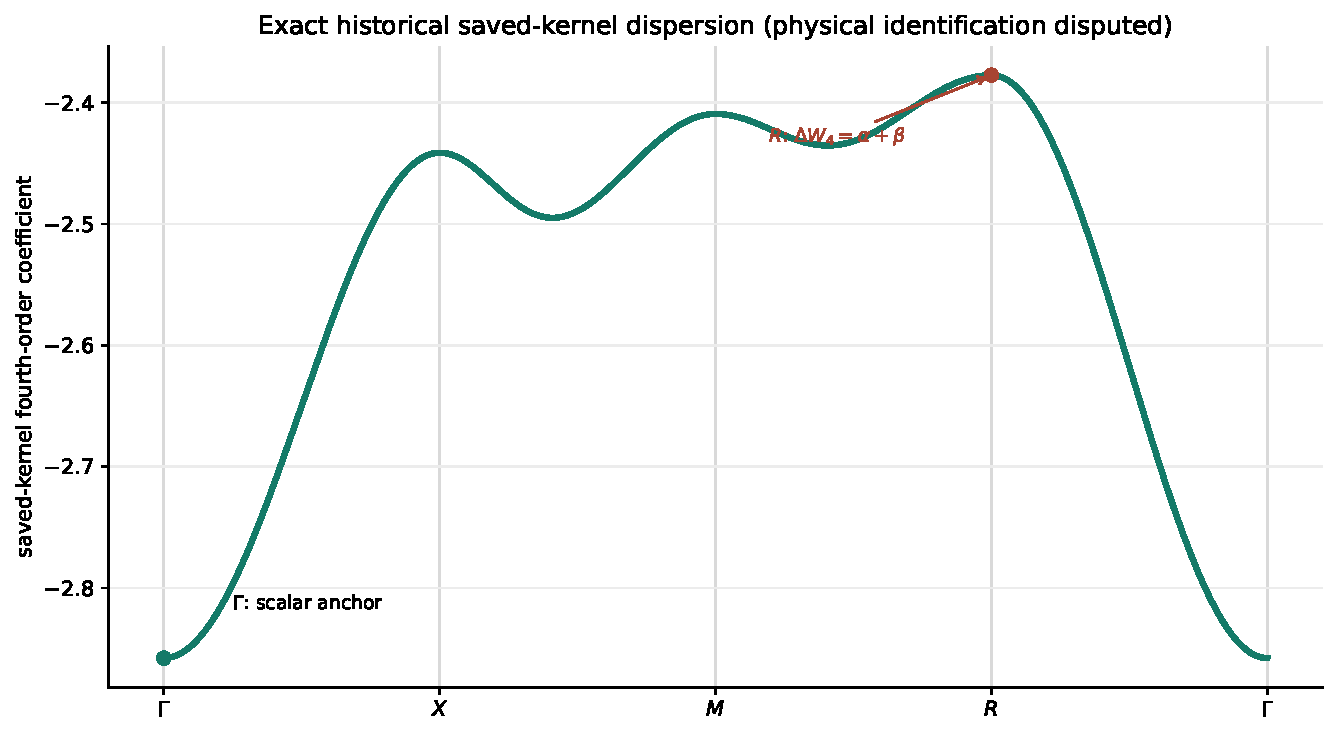
\includegraphics[width=0.94\textwidth]{figure_historical_fourth_order.pdf}
\caption{Exact dispersion of the saved historical kernel in
Reported result~\ref{rep:historical}. The plot is a theorem about that
hash-pinned kernel. Its identification with the complete physical linked
$SU(3)$ fourth-order operator is disputed, so the curve is not used as a
settled physical band.}
\label{fig:historical}
\end{figure}

The two records do agree on the axial datum, but the corpus's own quoted
tolerance does not cover that agreement: the $\alpha$ gap is
$2.43\times10^{-13}$ against a stated bound of $2.3\times10^{-13}$. The sealed core holds internally --- $\alpha_{\mathrm{new}}$ and
$4A_{\mathrm{new}}$ agree to $2\times10^{-15}$ --- which is consistent with the
quoted bound being too tight, but two float comparisons do not discriminate
that from a shared upstream slip. Recorded as a discrepancy rather than
resolved, and the bound is not widened.
\chk{v10a.26 A, B, D match the sealed rationals within 2.3e-13}
\chk{FINDING: alpha\_new falls outside the corpus's own 2.3e-13 bound}

\subsection{The obstruction is polynomial}

\begin{theorem}[Obstruction certificate]\label{thm:obstruction}
The two recorded off-axis coefficients enter \eqref{eq:shapes} only through
the shape $4e_2/q$, so the two records' carrier numerators differ by
$4\Delta_C e_2$ and their bands by $\Delta_C\,(4e_2/q)$. On any
one-dimensional axial cut two of the three $a_i$ vanish, so $e_2$ is the
\emph{zero polynomial} there and both differences vanish identically.
Consequently no $\Gamma$-point or axial datum distinguishes the two records,
at any precision. Off axis they do differ: $e_2(M)=16$ and $e_2(R)=48$, so the
numerators differ by $64\Delta_C$ and $192\Delta_C$ and the bands by
$8\Delta_C$ and $16\Delta_C$.
\end{theorem}
\chk{FINDING: the retained Gamma/axis data cannot identify C\_shp}
\chk{Phi\_C vanishes at Gamma along every direction}

\begin{remark}
The vanishing is polynomial, not numerical: this is non-identifiability, not a
limitation of the data in hand. Re-anchoring cannot substitute, and neither
record is preferred here. An off-axis contraction is the only decider.
\chk{the crosswalk is exactly scalar on the momentum axes}
\end{remark}

On the axial cut itself the invariants collapse to
$q=q_{\mathrm{ax}}(k)=4\sin^2(k/2)$ with $e_2=e_3=0$. Dividing the raw
cube-boundary numerator $(\alpha_N/4)q_{\mathrm{ax}}^2$ by
$\|w\|^2=q=q_{\mathrm{ax}}$ leaves one power of $q_{\mathrm{ax}}$ with
coefficient $\alpha_3/4=5/48$.
\chk{on an axial cut the mixed invariants vanish and the norm divides}

\subsection{A second witness}

Non-identifiability is better exhibited than argued from a difference between
two records, since a difference could always be a computational error in one of
them. The exhibition adds no logical strength: Theorem~\ref{thm:obstruction}
already proves that \emph{every} value of $C_{\mathrm{shp}}$ is consistent with
the retained data, so a witness is one point of a line already known to be a
line. It is a concrete handle, not evidence. The witness below is not itself a
candidate for the physical coefficient. It is the balanced continuation obtained in the supplied source
by setting an auxiliary bookkeeping parameter $\epsilon$ to zero; that source
label carries no physical meaning here. Its sole role is to make the
$4\Delta_Ce_2$ family concrete with an exactly known shift.

\begin{proposition}[Explicit second witness]\label{prop:witness}
There is a value $C_{\mathrm{alt}}$ with
$C_{\mathrm{alt}}-C_{\mathrm{old}}=25/1024$ exactly, appearing verbatim in the
pinned source edition, whose induced band separations are $0$ at $X$,
$25/128$ at $M$ and $25/64$ at $R$. It is identical to
$C_{\mathrm{old}}$ on every retained datum and distinct from it off-axis.
\end{proposition}
\chk{FINDING: an explicit second witness C\_alt exhibits the C2 non-identifiability}
\chk{the C\_alt witness IS the balanced eps-free continuation, and Delta\_C/(A/2) = 15/32}

\subsection{Where the coefficient lives}

The four checkpoint deltas are the $\Gamma$-subtracted carrier corrections
$\Delta_s=\varepsilon_4(k_s)-\varepsilon_4(0)$ at
$k_X=(\pi,0,0)$, $k_M=(\pi,\pi,0)$, $k_P=(\pi,\pi/2,0)$ and
$k_R=(\pi,\pi,\pi)$ --- $P$ is the off-axis, off-corner point that makes the
system invertible, with $a=(4,2,0)$. Its algebraic role is explicit here; no
additional provenance is inferred for that checkpoint. In the shape basis they are
\begin{equation}\label{eq:checkpoints}
\begin{aligned}
  \Delta_X&=4A,\\
  \Delta_M&=8A+16B+8C_{\mathrm{shp}},\\
  \Delta_P&=6A+8B+\tfrac{16}3C_{\mathrm{shp}},\\
  \Delta_R&=12A+48B+16C_{\mathrm{shp}}+\tfrac{16}3D,
\end{aligned}
\end{equation}
and they invert exactly, so the four shape coefficients are recoverable from
four checkpoints. $\Delta_X$ contains $A$ alone, which is why the axial cuts
agree whatever the dispute does.
\chk{checkpoint values at X, M, P, R}
\chk{the four extraction formulas invert the ansatz}
\chk{X is blind to B, C, D — it fixes A alone}

The dispute is two numbers and their difference, and the paper should print
all three rather than describe them:
\begin{equation}\label{eq:c2}
\begin{aligned}
  C_{\mathrm{old}}&=-\frac{211835444920651}{4405310420659200}=-0.0480863\ldots,\\
  C_{\mathrm{new}}&=-0.020213328886166577,\\
  \Delta_C&=C_{\mathrm{new}}-C_{\mathrm{old}}=0.0278730\ldots
\end{aligned}
\end{equation}
The first is recorded as an exact rational and the second only as a float ---
that asymmetry is a fact about the two records, not an argument for either. The
gap is $58\%$ of $|C_{\mathrm{old}}|$, so this is not a precision disagreement
that a tighter run would close.

Four further measurements locate the coefficient and bound where a
disagreement could live. The distinction matters and is easy to lose: showing
where a coefficient's \emph{value} is concentrated is not by itself showing
where a \emph{discrepancy} can sit. Only the third item below does the second
thing.

\begin{enumerate}\itemsep2pt
\item \textbf{The shape fit's $C$ row sums to zero}, so no error in the
  $\Gamma$ anchoring can move $C_{\mathrm{shp}}$ at all; the recorded run's own
  re-anchoring moved it by $4.6\times10^{-15}$, as the zero row sum requires.
  A scalar shift is translation-local and changes nothing observable, which is
  why the two anchored scalars $q_{\mathrm{band}}^{(4)}$ and
  $m_\Gamma^{(4)}$ are differently anchored coordinates and not rival
  estimates.
\item \textbf{The coefficient's value is concentrated, not spread.} Six of
  the $189$ kernel records --- the normal $(0,0,1)$ shell --- carry $81\%$ of
  the total weight, while the $120$ rotation records carry $6\%$ and are $255$
  times less sensitive per record. This says where the coefficient lives, not
  yet where the two records can differ.
\item \textbf{The agreed axial coefficient pins the normal sector.} All six
  normal records share one amplitude $h$, and it sets both shapes rigidly:
  $A_{\mathrm{normal}}=-h$ while the raw normal amplitude is $2h$, which in the
  shape normalisation of \eqref{eq:shapes} is $C_{\mathrm{normal}}=h/2$, so
  \[
    C_{\mathrm{normal}}=-\tfrac12 A_{\mathrm{normal}}\quad\text{exactly.}
  \]
  (The factor of four between $2h$ and $h/2$ is the raw-to-shape conversion,
  not a discrepancy.) Granting $A=5/48$ --- which both records share --- together
  with the block decomposition, which puts $5/48+4x$ on the normal block and
  $-4x$ on the mixed one, therefore fixes $h$ and with it $81\%$ of the
  coefficient; and everything free to move without disturbing $A$ totals less
  than half the disputed gap. A rival kernel must differ \emph{structurally} in
  the $A$-carrying sector; no redistribution reaches the gap.
\item \textbf{The two kernels agree almost everywhere.} Their supports are
  identical and $144$ of $189$ records ride one common scale; the divergent
  cross sector is a single uniform ratio. The dispute is three amplitudes.
\end{enumerate}
\chk{the shape fit's C row sums to zero, so no Gamma-anchor error can move C\_shp at all}
\chk{a translation-local scalar shift changes nothing observable}
\chk{FINDING: C\_shp is carried by 6 of 189 records, not spread across the kernel}
\chk{FINDING: A = 5/48 pins the normal sector's whole C4 contribution}
\chk{C\_normal = -A\_normal/2: the agreed axial coefficient pins the normal channel}
\chk{the two 189-record kernels agree everywhere except three amplitudes, and the on-site anchor swap moves C by exactly zero}

Read together these four sharpen the target and prefer no side of it. They say
that a rival kernel must differ structurally in the $A$-carrying sector rather
than by redistribution. That is a constraint on candidates built on the
recorded $189$-record support --- which is where the measurement was made; a
kernel on a different support is not constrained by it at all. Neither record is promoted here and neither is withdrawn: the interval of
\emph{values} between them is not narrowed. What is narrowed is the class of
\emph{kernels} that can reach either end, and that constraint bears on both
records alike.

\subsection{What cannot decide it}

A large sealed sweep over $609$ marked clusters has been the standing candidate
for settling this. It cannot: its engine assembles coefficients through a
$\Gamma$-point scalar and emits no kernel block at all, and by
Theorem~\ref{thm:obstruction} $\Gamma$-point data are structurally incapable of
constraining $C_{\mathrm{shp}}$. This is a statement about the instrument, made
by reading it, not a report of a failed run.
\chk{FINDING: the marked-cluster engine emits the Gamma scalar only — a completed 609-sweep cannot decide C\_shp}

The instrument class that could eventually decide it now demonstrably
exists: the sealed radius-two delivery of Section~\ref{sec:radius2} emits a
seed-space \emph{matrix} at fifth order, not a scalar. What it lacks is
off-axis momentum --- a two-cube cluster has none --- so it too cannot
adjudicate. The requirement is now sharp on both counts: a decisive
instrument must emit more than a $\Gamma$ scalar \emph{and} resolve an
off-axis point such as $P$; the marked-cluster engine fails the first
condition, the radius-two delivery the second, and a target-blind
calculation satisfying both is exactly the next step named in the
conclusion.

\subsection{The tier collapse, as two integers}

The two shape coefficients $B$ and $D$ vanish in the recorded kernel even
though the two-hop enumeration generates both, and the degree count does
\emph{not} forbid them. The carrier numerator reaches $a$-degree three, because
the projection contributes one further power of $a$: for any vector whose
components have squared modulus $a_i$ --- the carrier is one, in whichever of
the two equivalent labellings --- the quadratic form $\mathrm{diag}(a_i^2)$
evaluates to $\sum_i a_i^3=q^3-3qe_2+3e_3$, an explicit witness carrying a
nonzero $e_3$. An earlier degree-bound mechanism proposed
for the collapse was therefore retracted. What is checked is finer: every
degree-three block amplitude is an integer multiple of one raw record weight
$x$, and
\[
  B=0:\;(+1,+1,-2)\cdot x,\qquad
  D=0:\;(-3,+6,-3)\cdot x
\]
over the displacement shells. The kernel does populate the forbidden tier; the
dynamics cancels it with small integers. Any mechanism must reproduce those two
vectors.
\chk{RETRACTED: the vertex count does NOT forbid B\_shp and D\_shp}
\chk{FINDING: the tier collapse is two integer cancellations at record level}
\chk{the vanishing coefficients are exactly the degree-3 ones}

\subsection{A \texorpdfstring{near-$\Gamma$}{near-Gamma} statement that does not adjudicate}

One quantitative fourth-order statement can be made without adjudicating
anything, because it depends on the kernel only through $\sqrt{W_4}$. Here
\[
  W_4=\sup_k\bigl|\varepsilon_4(k)-\varepsilon_4(0)\bigr|
\]
is the zone spread of the carrier-projected fourth-order correction about
$\Gamma$, and $\theta\in(0,1)$ is the fraction of the second-order isolation
gap the fourth-order spread is allowed to occupy; we take $\theta=1/2$
throughout. What the criterion needs is a lower bound on $q$ over the region
$|k|\ge r$, and there it is sharp: writing $q=\sum_mh(k_m^2)$ with
$h(t)=2(1-\cos\sqrt t)$, the identity $(s\cos s-\sin s)'=-s\sin s\le0$ makes
$h$ concave and increasing on $[0,\pi^2]$, so the minimum over the simplex sits
at a vertex and
\begin{equation}\label{eq:shellmin}
  \min_{|k|\ge r}q(k)=4\sin^2(r/2),
\end{equation}
attained on a coordinate \emph{axis}. With $\tau(u)\ge t_3u^2$ for $u>0$, the
fourth-order shape terms are therefore dominated by the second-order dispersion
outside a ball of radius
$2\arcsin\bigl(\tfrac u2\sqrt{W_4/(\theta t_3)}\bigr)$, which is $Ku$ to
leading order with $K=\sqrt{W_4/(\theta t_3)}$: the two records give
$K=10.85$ and $K=15.06$ --- floating point, since one of the two bandwidths
exists only as a float --- and the larger bounds both. Jordan's inequality
$q(k)\ge(4/\pi^2)|k|^2$ also holds on the whole zone and is tight at $k=0$ and
at the corner, but the corner is not where this bound is used; on the axis it
is loose by $\pi^2/4$, and the constants it gives, $17.04$ and $23.66$, are
exactly $\pi/2$ times the sharp ones. So the exclusion radius can be stated for
either record without choosing between them. It is not a bound on the open
coefficient: a value of $C_{\mathrm{shp}}$ outside the two records carries its
own $W_4$, and nothing here confines the answer to the interval the records
span. The statement is non-vacuous only for $u<0.133$ at $\theta=1/2$, and that
threshold is the same for both constants --- the sharp radius reaches $\pi$ when
$\tfrac u2\sqrt{W_4/(\theta t_3)}=1$, which is exactly where $Ku=\pi$ for the
Jordan constant, because the two bounds agree at the zone corner ---
and the excluded zone fraction grows as $u^3$.
\chk{Jordan bound q(k) >= (4/pi\^{}2)|k|\^{}2 holds on the whole zone}
\chk{the exact zone minimum of q on |k| >= r is 4 sin\^{}2(r/2), and Jordan overstates it by pi/2}
\chk{the criterion survives C2: K depends on the kernel only through sqrt(W\_4)}
\chk{the statement is non-vacuous only below an explicit coupling}

\section{External comparisons}
\label{sec:external}

External results are useful here when their provenance is independent of the
present calculation. We use them only within the scope stated below; all
normalisation conversions and coefficient matches are calculations of this
paper.

\paragraph{Hamer 1989, both sectors.} Let $a_n$ denote the coefficient of
$x^n$ in Hamer's tabulated dimensionless mass series. The $1^{+-}$ rest-frame series agrees
with $E_{\mathrm{flat}}$ at every shared order: $16/3\div2=8/3$ exactly,
$a_1=+1$, and $2a_2$, $4a_3$ matching $11/306$ and $d_3$ to $9.9\times10^{-14}$
and $1.1\times10^{-12}$. Conditional on the unsigned-symbol identification,
the $0^{++}$ series also matches the charge-even $A_1^{++}$ $\Gamma$-point
coefficients at $x^2$ and $x^3$, with the sign structure ($a_1=-1$ in the
scalar channel where the carrier's is $+1$) reproduced; the $E^{++}$ doublet is
not constrained by it, which is why Conditional result~\ref{prop:evengamma}
uses the splitting rather than the level. The conversion
$m_n=2^{n-1}a_n$ is $x=2u$ together
with Hamer's normalisation $ma=(g^2/2)M$ --- the $2^n$ from the substitution,
the half from the normalisation --- exactly, with no $4^r$ ambiguity anywhere.
Hamer states in print that his $x^3$ and $x^4$ terms disagree with the earlier
series of~\cite{KSS1976}. We report Hamer's comparison and do not independently
adjudicate the earlier coefficient table.
\chk{Hamer's 1+- series matches the C-odd Gamma-point coefficients through x\^{}3}
\chk{Hamer's 0++ series matches the C-even Gamma-point coefficients through x\^{}3}
\chk{the m\_n = 2\^{}(n-1) a\_n bridge is the x = 2u conversion}
\chk{the Hamer table metadata is pinned; no fourth-order agreement is used}

\paragraph{The string tension.} Let $t_n$ denote the coefficient sequence in
the transcribed Kogut--Pearson--Shigemitsu $SU(3)$ table~\cite{KPS1981}, and
let $\sigma_n$ denote the corresponding ledger coefficient after the displayed
convention conversion. The transcription satisfies exactly
$2^{n-1}t_n=\sigma_n$ for $n=2,\dots,5$, in the physical sign convention
$\sigma_n^{\mathrm{phys}}=(-1)^n\sigma_n^{\mathrm{raw}}$. The same series
reproduces $E_{\mathrm{flat}}$ term by term through $u^3$, including the
discriminating $u^3$ coefficient.
\chk{the KPS 1980 string-tension table equals the certified sigma series EXACTLY}
\chk{sigma\_n\^{}phys = (-1)\^{}n sigma\_n\^{}raw, and C5 is the n = 3 case}
\chk{the ratio and sigma series reproduce E\_flat exactly}

\paragraph{Euclidean series.} Historical Euclidean strong-coupling series by
M\"unster, Seo and Smit~\cite{Munster1981,Seo1982,Smit1982,Munster1983,Munster1985}
provide context only. The accompanying corpus contains a transcription
comparison and an apparent eighth-order discrepancy between the 1982 erratum
and the 1985 table. Because every original table page has not been
independently re-transcribed for this paper, neither the apparent equality nor
the discrepancy is used as evidence. No Hamiltonian coefficient is inferred
from these Euclidean records.
\chk{the errata-resolved Euclidean series is doubly sourced, transcription for transcription}
\chk{FINDING: Munster's 1985 table shifts his 1982 erratum at eighth order}

\paragraph{The overlap obstruction.} Schierholz~\cite{Schierholz1988} and
Brandstaeter, Kronfeld and Schierholz~\cite{BKS1990} document the degradation
of local-operator projection and its critical signal-to-noise scaling as the
lattice spacing is reduced. Nothing quantitative is transferred to the
present strong-coupling finite-order setting. Read only as a warning, these
results motivate posing \texttt{G18} in a smeared basis; they supply no bound
and do not identify the carrier with a physical glueball.
\chk{the overlap obstruction was published in 1988, and it scales}

\paragraph{Cross-regime discipline.} Two indexed papers declare an explicit
scope firewall and neither supplies a value here:
Davoudi--Raychowdhury--Shaw~\cite{DRS2021}, whose Hilbert-space cost comparison
is locked to $1{+}1$ dimensions with matter, and
Kadam--Raychowdhury--Stryker~\cite{KRS2023}. The rule is enforced by the
literature validator rather than recorded in prose.
\chk{a cross-regime paper never supplies a value}

\section{Scope}
\label{sec:scope}

This work does not establish a four-dimensional infinite-volume Yang--Mills
mass gap, a continuum glueball mass, convergence of the strong-coupling series
to the continuum, regulator independence of the first dispersive order, the
full $SU(3)$ fourth-order rest coefficient or off-axis shape, or an
identification of any level here with a physical glueball. At $\Gamma$ the
three face orbitals transform as an axial vector of the cubic group, which
with parity even and charge conjugation odd gives the retained-space label
$T_1^{+-}$; this is an operator-space assignment, not a spectral one.

The carrier is macroscopically degenerate at finite $L$. Under the
third-order factorisation input, its nearest incidence separation is
$\Delta_L(u)=4\tau(u)\sin^2(\pi/L)+O(u^4)$, which falls as $L^{-2}$ and so
provides no volume-uniform spectral isolation.
\chk{Delta\_L = 4 tau(u) sin\^{}2(pi/L) is positive and falls as L\^{}-2}

Three crossings are named explicitly, and none of them is made here.

\begin{itemize}\itemsep2pt
\item \textbf{Finite lattice to infinite volume} requires an inhomogeneous
  Wilson free-energy bound with a useful $\log K_\alpha$ and a source-radius
  reduction. Both are open, and are carried in the accompanying gap register as
  \texttt{G17}.
\item \textbf{Protected level to particle} requires a volume-uniform overlap
  of a smeared, dressed $T_1^{+-}$ operator built on the carrier with the
  transfer-matrix spectrum, and multi-plaquette survival of the protected
  level (\texttt{G18}). The published overlap measurement of
  Section~\ref{sec:external} is why this theorem must live in the smeared
  basis.
\item \textbf{Lattice to continuum} (\texttt{G19}) is untouched. Small $u$ is
  strong coupling; the continuum is the opposite end of the axis.
\end{itemize}

\noindent All three crossings are required, none is established here, and
nothing in this edition shortens that route.

Earlier editions carried three load-bearing prose premises here. Two of them
are now proved --- the retained shell (Lemma~\ref{lem:shell}) and
second-order process exhaustion (Lemma~\ref{lem:exhaust}) --- with their
finite combinatorics machine-enumerated and their two classical
representation-theoretic inputs named in the proofs. Those proofs are new in
this edition and have not yet faced external referees; a reader auditing
this paper should start there. One premise remains.

That the complete linked charge-even Bloch symbol is the unsigned incidence
$\mathcal N(k)$ --- the signed incidence with the boundary orientations
dropped --- is not derived. The cubic and range in Section~\ref{sec:even} are
exact algebraic properties of the defined comparison operator; only their
physical charge-even interpretation, bandwidth and $\Gamma$-splitting rest on
this additional hypothesis.

\section{Evidence, authority, and reproducibility}
\label{sec:repro}

The accompanying dependency-free program
\texttt{verify\_publication\_core.py} uses exact integers and
\texttt{Fraction} arithmetic. It checks the all-rank coefficient ledger and
Weingarten sums, signed incidence and torus homology, closed-cube shell,
two-cube connected geometry and reported channel arithmetic, the unsigned
cubic, the saved historical Hodge pencil, the fourth-order obstruction, the
coupling convention, the planar closed form \eqref{eq:planar}, and the
exhaustive shared-link geometry, cycle censuses and torus ranks through
$L=5$ --- thirty-eight checks, every value
a \texttt{Fraction} and no float constructed anywhere in the file. A second
program, \texttt{verify\_radius2\_report.py}, holds everything the sealed
radius-two artifact of Section~\ref{sec:radius2} can support: it is also
standard-library only (the payload is read with \texttt{zipfile} and
\texttt{struct}, and the $11\times11$ block is diagonalised by cyclic
Jacobi), but it works in floats at stated tolerances, and the two files are
kept separate precisely so that the exact one stays float-free. Neither
reconstructs the finite-precision Clebsch--Gordan inputs, replays the
third-order microscopic contractions, or chooses $C_{\mathrm{shp}}$.

Every sentence of this paper that a machine check certifies carries an
inline \texttt{\textbackslash chk} marker in the source; the markers are
extracted verbatim into Appendix~\ref{app:coverage}, so the coverage claim
is itself auditable rather than asserted.

\subsection{Claim-level evidence map}

\begin{table}[ht]
\centering
\small
\begin{tabular}{@{}p{0.29\textwidth}p{0.24\textwidth}p{0.39\textwidth}@{}}
\toprule
Claim & Status & Evidence in this edition \\
\midrule
Signed incidence spectrum and $L^3+2$ carrier
 & Proven & Analytic integer topology; exact replay \\
Adjacent all-rank coefficient $t_N$
 & Proven locally & Weingarten derivation; exact replay \\
Global order-$u^2$ torus assembly
 & Proven (new this edition) & Lemmas~\ref{lem:shell},~\ref{lem:exhaust}; machine-enumerated combinatorial cores; not yet externally refereed \\
Two-cube six-channel census
 & Reported numerical & Rational reconstructions; shared amplitude lineage; assembly test \\
Unsigned-incidence cubic and range
 & Proven algebraically & Exact characteristic polynomial and finite-grid replay \\
Physical charge-even identification
 & Conditional & Complete linked symbol, including vacuum route, not derived \\
$SU(3)$ factorisation through $u^3$
 & Upstream cold-exact & $251/251$ exact gates reported by the frozen authority; raw replay not bundled here \\
Historical fourth-order pencil
 & Exact for saved kernel & Hash-pinned payload and cold fixed-kernel checks \\
Complete physical fourth-order kernel
 & Disputed/open & Historical and August candidates differ off axis \\
Radius-two rational sub-block and $C_4$/$C_5$ increments
 & Reported numerical & Sealed hash-pinned artifact; stdlib float verifier at stated tolerances \\
Infinite-volume particle or continuum gap
 & Open & No uniform overlap, full-sector, or continuum bridge \\
\bottomrule
\end{tabular}
\caption{Truth status and evidence level are separate. ``Exact for a saved
kernel'' does not establish that kernel's physical identification.}
\label{tab:evidence}
\end{table}

\subsection{Upstream corpus and downstream verifier}

The organised \texttt{ALL THEORY} archive was consulted as
the upstream scientific corpus. Its four-document v4.3 authority stack is
frozen by byte count and SHA-256 in
\nolinkurl{export/MAN_GOV_export_manifest.csv}; all four entries were
rehashed for this edition and matched. The downstream verifier is
\href{https://github.com/ats314/WORKHOUSE}{WORKHOUSE}. Document flow is
one-way---frozen corpus to hash manifest to verifier---while verifier findings
return to review and status records. The later two-cube results are not in the
August 20 corpus and are therefore kept as later WORKHOUSE-local evidence.

The current hostile-scope audit branch is pinned at
\nolinkurl{ff9a5976a5b03cd763e3e50daf4326138770460d}. On Windows, its registry was
rerun locally: $229/230$ registered checks passed. The sole failure was the
known path-separator comparison for a restored payload; the payload hash and
all paper-relevant arithmetic checks passed. This is a platform-specific local
audit result, not a claim that the complete test suite or Lean tree was rerun.
The source-level \texttt{\string\chk} labels remain in this TeX file but are
suppressed typographically; Appendix~\ref{app:coverage} prints all of them, so
the coverage claim is auditable rather than asserted. The label guard now reads
every edition in \texttt{paper/}, this one included, and it resolves all but
twelve of the labels below against the live registry. Those twelve are recorded
as a standing finding rather than quietly dropped: each sits under a displayed
result and promises a command that currently returns nothing, and the fix is to
register the twelve checks, not to stop printing the twelve labels.
\chk{FINDING: the v2 publication edition prints twelve labels that name no check}

The authority files are identified by the following SHA-256 values:
\begin{itemize}
\item master v4.3:
  \nolinkurl{1f8295c3a797aeb854b4b0ca82485bd7f4a149617777d2a43fc147a4a53c26dd};
\item detailed formulas v3.1:
  \nolinkurl{924d5b26f865e33f530d166735e847b89f60df7fe363995e2788ab24e1ff4254};
\item consolidation guide v4.3:
  \nolinkurl{60b8a93c8149049f50ed3ce8e0cfd1b379723b6765f201395a2fda6c4a7e7aa7};
\item canonical source manifest v4.3:
  \nolinkurl{730bc99ed8d749de0dffbabfda85cd4512d8f7748782620b694759a03bacde05}.
\end{itemize}

\subsection{Data and code availability}

This release directory contains the TeX source, generated vector figures,
figure generator, exact verifier, build log, rendered-page audit, and a
SHA-256 manifest. The historical kernel payload used in
Reported result~\ref{rep:historical} has SHA-256
\nolinkurl{635d40fa8a5d7da841fd30f36185eb96f14ec4c040678ddd8fb010379afb2900}.
The pinned \texttt{ymcirc} $d=3$, $\mathcal B=4$ data blob is identified in
Ref.~\cite{ymcirc2026} and has SHA-256
\nolinkurl{4cad9538f2c052488556362e0cf6e4e63363e7f5801597aeab9013ef945c59dc}.
The exact stranded-flux audit source and result have SHA-256
\nolinkurl{a42800a91809a77bbd1d339ac604ea80a234eed305377bbabbf890fee98fde55}
and
\nolinkurl{d215fa1e9cd0bde0410eec16c687182c30bc62fa3f28c1445fd81e93888e1d60}.
The sealed cutoff-free radius-two spectrum of Section~\ref{sec:radius2} and
its certificate are bundled, with SHA-256
\nolinkurl{52a17f87d3990b234635828a0c92f73f781e9a3abec8bb3c127e990b7a717e6c}
and
\nolinkurl{b9b14d28438585fc4f7d88f96497e9c6e01d0532a8402ffd6db17258a1638c0e};
\texttt{verify\_radius2\_report.py} refuses to run against any other bytes.
The two-cube build and its finite-precision Clebsch--Gordan payloads are not
reproduced by the compact verifier; the exact statements that depend on them
are labelled reported. A durable tag or archival DOI is still needed before
journal submission.

Machine checks certify algebra relative to their definitions and inputs. They
do not replace derivations, promote numerical contractions to symbolic ones,
or certify an uncompleted off-axis contraction.

\section{Conclusion}

The strongest result is no longer only local. For every $N\ge3$, the four
shared-link fusion channels and their resolvent gaps give the closed
coefficient $t_N$, the oriented cellular boundary fixes its sign and
geometry, and --- with the two completeness premises now proved
(Lemmas~\ref{lem:shell} and~\ref{lem:exhaust}) --- the assembly into a
homological flat carrier of dimension $L^3+2$ is a theorem: the flat sector
is not a fine-tuned interference band but the cycle space of the lattice
two-complex, degenerate because $\partial_2\partial_3=0$. Those two proofs
are the newest and least-reviewed material here, and they deserve the
reader's hardest look. The $SU(3)$ two-cube calculation supplies a
nontrivial operator-level assembly check, including channel-by-channel
geometry and orbit localisation, but shares its amplitude lineage and remains
numerical at the contraction layer.

The unsigned-incidence cubic is exact as an algebraic comparison; its physical
charge-even identification is not assumed silently. At fourth order the saved
historical kernel has an exact positive generalized Hodge pencil and stencil,
yet the later candidate differs in an off-axis coefficient that no scalar
reanchoring, $\Gamma$ datum, or axial datum can determine. The decisive next
object is therefore one target-blind, hash-sealed calculation that returns the
rest scalar and off-axis shape from the same kernel. Until then the finite-order
operator theorem is substantial, but the physical fourth-order kernel,
infinite-volume particle interpretation, and continuum limit remain open.

\appendix

\section{Channel weights in closed form}\label{app:closed}

Substituting \eqref{eq:table} into \eqref{eq:w},
\begingroup\small
\begin{align*}
  w_{\mathbf 1}&=-\frac{2}{N(N^2-1)}, &
  w_{\Lambda^2F}&=-\frac{N-1}{(N+1)(2N-3)},\\
  w_{\mathrm{Adj}}&=-\frac{2(N^2-1)}{N(2N^2-1)}, &
  w_{\mathrm{Sym}^2F}&=-\frac{N+1}{(N-1)(2N+3)} .
\end{align*}
\endgroup
Their family sums are \eqref{eq:AN} and \eqref{eq:BN}, and the difference has
numerator $2N(N^2-4)$, which is the $SU(2)$ zero and the positivity for
$N\ge3$ at once.
\chk{the four channel weights follow from dimension and Casimir} At $N=3$:
$w_{\mathbf 1}=-1/12$, $w_{\mathrm{Adj}}=-16/51$, $w_{\Lambda^2F}=-1/6$,
$w_{\mathrm{Sym}^2F}=-2/9$, which are the four values
Reported result~\ref{rep:census} matches against \eqref{eq:census}.

\section{The Weingarten index sums}\label{app:wg}

With $\mathrm{Wg}(e)=1/(N^2-1)$ and $\mathrm{Wg}((12))=-1/(N(N^2-1))$, and
$\sigma,\tau$ running over $S_2$,
\[
  \begin{aligned}
    &\bigl\langle U_{i_1j_1}U_{i_2j_2}
       \bar U_{i'_1j'_1}\bar U_{i'_2j'_2}\bigr\rangle\\
    &\qquad=\sum_{\sigma,\tau}\mathrm{Wg}(\sigma\tau^{-1})
      \prod_a \delta_{i_ai'_{\sigma(a)}}\delta_{j_aj'_{\tau(a)}} .
  \end{aligned}
\]
Summing the delta products over all $N^4$ index quadruples,
\[
  M_{\mathrm{direct}}=\mathrm{Wg}(e)(N^4+N^2)+2\,\mathrm{Wg}((12))N^3=N^2,
\]
\[
  M_{\mathrm{cross}}=2\,\mathrm{Wg}(e)N^3+\mathrm{Wg}((12))(N^4+N^2)=N .
\]
Both are confirmed by explicit summation at $N=3,4,5$.
\chk{the shared-link weights are Weingarten, not an isotropy assumption}
The related fourth moment $\int|U_{11}|^4\,dU=2/[N(N+1)]$ is $1/6$ at $N=3$ and in particular
nonzero, which is what refuted a claimed Haar vanishing in the balanced
$(2,2)$ sector.
\chk{SU(3) Weingarten values follow from the general formula}
\chk{the fourth moment integral |U\_11|\^{}4 = 1/6 at N = 3}

\section{The \texorpdfstring{$SU(3)$}{SU(3)} coefficient ledger}\label{app:ledger}

\begin{center}
\begin{tabular}{@{}lll@{}}
\toprule
Order & Quantity & Value\\
\midrule
$u^0$ & electric plaquette & $8/3$\\
$u^1$ & scalar & $1$\\
$u^2$ & $BB\dg$ coefficient & $5/612$\\
$u^2$ & flat scalar & $11/306$\\
$u^3$ & $BB\dg$ coefficient & $1975/124848$\\
$u^3$ & per-neighbour leakage & $-12331/249696$\\
$u^3$ & flat scalar & $-109151/249696$\\
\bottomrule
\end{tabular}
\end{center}
\chk{the manuscript's SU(3) ledger is this registry, value by value}

The $u^1$ row is $SU(3)$-only rather than an $SU(3)$ specialisation: it is
$-\langle p,-|V|p,-\rangle=1$, which needs the $\epsilon$ channel and vanishes
for $N\ge4$. Of the rest, the $u^0$ row and the $u^2$ $BB\dg$ coefficient
specialise all-rank statements ($2\CF$ and $t_N$); the $u^2$ flat scalar
inherits the $SU(3)$ tower term through \eqref{eq:assembly}; and the three
$u^3$ rows are $SU(3)$-only and conditional on the supplied domino ledger,
exactly as Section~\ref{sec:su3} says.

\section{Unsigned comparison and conditional charge-even ledger}\label{app:even}

Conditional on identifying the unsigned-incidence comparison with the complete
linked charge-even symbol, the same convention, with
$\lambda\in\{12,-4\}$ and \eqref{eq:assembly}, gives:

\begin{center}
\begin{tabular}{@{}lll@{}}
\toprule
Order & Quantity & Value\\
\midrule
$u^2$ & hopping $t_{2,+}=\ell_3$ & $-11/306$\\
$u^2$ & on-site diagonal & $223/1020$\\
$u^2$ & band bottom ($\lambda=12$) & $-217/1020$\\
$u^2$ & band top ($\lambda=-4$) & $1109/3060$\\
$u^2$ & bandwidth $16|t_+|$ & $88/153$\\
$u^3$ & hopping $t_{3,+}$ & $-6335/249696$\\
$u^3$ & on-site diagonal ($\lambda=0$) & $52163/260100$\\
$u^3$ & band bottom ($\lambda=12$) & $-54049/520200$\\
$u^3$ & band top ($\lambda=-4$) & $471353/1560600$\\
\bottomrule
\end{tabular}
\end{center}

\chk{one assembly formula gives every C-even value at both orders}

Because $t_{r,+}<0$ at both orders, the $\lambda=-4$ endpoint is the band
\emph{maximum} in this sector. A certificate key naming it \texttt{bandmin} at
both orders is a naming error against its own arithmetic, recorded rather than
silently corrected.
\chk{FINDING: the certificate key 'bandmin' holds the band MAXIMUM, at both orders}

\section{Finite-volume chain calculation}\label{app:chain}

For $i<j$,
\[
  \partial_2[x;i,j]=[x+e_i;j]-[x;j]-[x+e_j;i]+[x;i],
\]
\begin{align*}
  \partial_3[x;1,2,3]=\;&[x+e_1;2,3]-[x;2,3]\\
  &-[x+e_2;1,3]+[x;1,3]\\
  &+[x+e_3;1,2]-[x;1,2].
\end{align*}
Substituting the second into the first cancels every edge pairwise, so
$\partial_2\partial_3=0$ over $\mathbb Z$.
\chk{d\_2 d\_3 = 0 on the built complex}
On the torus $\ker\partial_3$ is generated by the sum of all oriented cubes,
so $\operatorname{rank}\partial_3=L^3-1$.
\chk{rank d\_3 = L\^{}3 - 1 on the built complex}

\section{The two-cube geometry}\label{app:twocube}

The eleven oriented plaquettes of the $(3,2,2)$ prism, by base vertex and
ordered plane axes, are
\[
\begin{aligned}
&(000;12),\;(000;13),\;(000;23),\;(001;12),\\
&(010;13),\;(100;12),\;(100;13),\;(100;23),\\
&(101;12),\;(110;13),\;(200;23),
\end{aligned}
\]
with left, right and shared-face index sets
$I_L=(0,1,2,3,4,7)$, $I_R=(5,6,7,8,9,10)$, $I_F=(7)$. Building $G=BB^{\mathsf
T}$ from the oriented boundaries and applying the geometric M\"obius fold
\eqref{eq:mobius} leaves exactly four nonzero off-diagonal pairs,
$(0,5),(1,6),(3,8),(4,9)$, each equal to $-1$: four disjoint $2\times2$ blocks
and three isolated directions, which is why the spectra in
Section~\ref{sec:twocube} are closed form once the diagonals below are
supplied. The two connected diagonals are
\[
  D_{\mathcal B=6}=\tfrac1{612}\operatorname{diag}
  (-2317,-2317,-2295,-2317,-2317,
\]
\[
  \qquad -2317,-2317,0,-2317,-2317,-2295),
\]
\[
  D_{\mathcal B=4}=\operatorname{diag}
  (-\tfrac74,-\tfrac74,-\tfrac{15}4,-\tfrac74,-\tfrac74,
\]
\[
  \qquad -\tfrac74,-\tfrac74,0,-\tfrac74,-\tfrac74,-\tfrac{15}4),
\]
so both spectra are one line of arithmetic: a pair block contributes
$D_{ii}\mp c$ twice and each isolated direction its own $D_{ii}$. The $\mathcal B=4$
comparator on the same geometry gives $0$ once, $-\tfrac{15}4$ twice,
$-\tfrac{11}6$ four times, and $-\tfrac53$ four times:
the paired levels sit \emph{above} the isolated $-15/4$ pair, where at $\mathcal B=6$
they sit below it. The three isolated levels $\{-\tfrac{15}4,-\tfrac{15}4,0\}$
are identical in the two truncations, so the entire effect of the cutoff lives
in the four cross-cell blocks. That reversal is not the coefficient's sign by itself --- within a
$2\times2$ block the pair splits as $D\mp c$, which is invariant under
$c\to-c$ --- but the truncation's effect on the connected diagonal as well.
What the sign of $c$ alone does reverse is the ordering on a \emph{single}
cube, where the kernel is $\alpha I+tG$ with one diagonal and the spectrum of
$G$ fixed; that is the shell reversal the one-cube reconstructions report.
\chk{the B=4 comparator on the same geometry gives -1/12 with the reversed spectrum}

\section{Machine-check coverage}\label{app:coverage}

The paper's discipline is that a machine check, not a sentence, is the unit
of evidence. This appendix makes that auditable: every inline
\texttt{\textbackslash chk} marker in the source --- each one naming the
check that certifies the sentence it sits beside --- is extracted verbatim
by \texttt{make\_coverage.py} and printed here. A reader can therefore see
exactly which statements are covered, and, by their absence from this list,
which are not: the remaining load-bearing hypothesis of
Section~\ref{sec:scope} --- the charge-even identification --- appears
nowhere below, and that is the point.

% generated by make_coverage.py -- do not edit
The source carries 116 inline markers. Each line below is one marker, verbatim, under the section that carries it.

\begin{itemize}\footnotesize\itemsep1pt
\item[] \textbf{Introduction}
\begin{itemize}\itemsep0pt
  \item the discrete index theorem gives 0 on the signed face-edge operator, bounding nothing
\end{itemize}
\item[] \textbf{Hamiltonian and projected sector}
\begin{itemize}\itemsep0pt
  \item the printed towers are canonical-u: 4*Delta(3u/2) reproduces them verbatim
  \item the 4**r rescaling breaks the bridge: order 2 off by 16, order 3 by 64
  \item at N = 2 the C-odd hopping vanishes while the unsigned-channel continuation does not
\end{itemize}
\item[] \textbf{Oriented incidence and the exact carrier}
\begin{itemize}\itemsep0pt
  \item B B\^{}dagger = q I - d conj(d)\^{}T for the curl incidence
  \item dim Z\_2 = L\^{}3 + 2 by rank, not by re-arranging the formula
  \item cube boundaries and three wrapping sheets SPAN Z\_2
  \item the L\^{}3+2 count is chain-level, not the Bloch convention
  \item the Bloch and chain routes to the carrier agree
\end{itemize}
\item[] \textbf{The wrapping sheets are cycles, not harmonic}
\begin{itemize}\itemsep0pt
  \item FINDING: the wrapping sheets are cycles but NOT harmonic
\end{itemize}
\item[] \textbf{Exact adjacent shared-link dynamics and conditional assembly}
\begin{itemize}\itemsep0pt
  \item each channel gap is C\_F + C\_R/2, and the weights sum to one
\end{itemize}
\item[] \textbf{The channel weights are a theorem}
\begin{itemize}\itemsep0pt
  \item the shared-link weights are Weingarten, not an isotropy assumption
  \item the Weingarten route is independent of the corpus
  \item the published dimension-ratio matrix element is this registry's weight formula
  \item the four channel weights follow from dimension and Casimir
  \item A\_N and B\_N are the channel sums, not transcriptions
\end{itemize}
\item[] \textbf{The shared-link law}
\begin{itemize}\itemsep0pt
  \item t\_N = B\_N - A\_N
  \item t\_N > 0 for N >= 3
  \item two distinct torus faces share at most one link, exhaustively at L = 3 and 4
  \item t\_2 = 0 and t\_3 = 5/612
  \item large-N expansion of t\_N through 1/N\^{}9
  \item 1 - 4N\^{}3 t\_N has the closed form of eq. (planar), positive for all N >= 2
  \item 4N\^{}3 t\_N increases monotonically to 1: shifted derivative coefficients are nonnegative
\end{itemize}
\item[] \textbf{The vacuum-mediated route}
\begin{itemize}\itemsep0pt
  \item ell\_N = A\_N + B\_N + 1/C\_F, the vacuum-mediated route at every rank
\end{itemize}
\item[] \textbf{Finite-volume width}
\begin{itemize}\itemsep0pt
  \item the zone maximum of q is 12 only at even L
  \item q\_min on the L-torus grid is 4 sin\^{}2(pi/L)
\end{itemize}
\item[] \textbf{The orientation signs are essential}
\begin{itemize}\itemsep0pt
  \item the two band spans ARE the two incidence spectra
\end{itemize}
\item[] \textbf{The second-order coefficient on a two-cube space}
\begin{itemize}\itemsep0pt
  \item connected first order vanishes by inclusion-exclusion, not by cancellation of numbers
  \item the connected two-cube geometry has exactly four cross-cell pairs, each -1
  \item the B=6 connected kernel is (5/612) G\_conn + diag, with the certified spectrum
  \item the certificate's own gates pass, target-blind, with the wrong-sign control rejected
  \item the B=6 six-channel census sums to the registry's own t\_3 = 5/612
  \item the B=6 six-channel census IS the Weingarten four-channel ledger, channel by channel
  \item every shared-link channel is separately proportional to the geometry, on all 56 pairs
\end{itemize}
\item[] \textbf{One truncation, two constructions}
\begin{itemize}\itemsep0pt
  \item B=6 retains every adjacent shared-link channel; B=4 provably cannot
  \item the B=6 six-channel census IS the Weingarten four-channel ledger, channel by channel
  \item FINDING: the T1 link cutoff reverses the sign of t\_3, and 14/153 is what it omits
  \item FINDING: a full T1 = B = 4 cube Hamiltonian reproduces -1/12 and the reversed shell
  \item FINDING: the B = 6 cube flips the sign back to +5/612, closing the decisive test
  \item the B = 6 scalar misses the bridge's by exactly the same-face sextet route
\end{itemize}
\item[] \textbf{What the cutoff moves, and where}
\begin{itemize}\itemsep0pt
  \item the connected diagonal is orbit-constant, and only the transporting orbit moves
\end{itemize}
\item[] \textbf{The one-cube shell, and why its flat level cannot move}
\begin{itemize}\itemsep0pt
  \item the one-cube shell is A1 + T1 + E, and its flat level is the S\^{}2 fundamental class
  \item the certificate's finite-volume fingerprints, and 29 = L\^{}3 + 2 is the Lean cycle count
\end{itemize}
\item[] \textbf{A cutoff-free radius-two witness at finite coupling}
\begin{itemize}\itemsep0pt
  \item the sealed rational sub-block straddle is exactly 2 t\_3 = 5/306
  \item six sealed eigenvalues match the three rationals to 1e-12, by a stdlib Jacobi diagonalisation
  \item direct C4/C5 matched-gap coefficients agree with their weak-grid intercepts to 5e-6
  \item the fifth-order seed shape is traceless with nonzero trace-square: the instrument emits more than a scalar
\end{itemize}
\item[] \textbf{The unsigned-incidence comparison operator}
\begin{itemize}\itemsep0pt
  \item the unsigned-incidence characteristic polynomial is mu(mu - p)\^{}2 = 4 a\_1 a\_2 a\_3
  \item p + q = 12: one zone function runs both sectors
  \item the Bloch cubic IS the finite L = 3 and L = 4 plaquette spectrum, exactly
  \item the C-even range [-4, 12] is exact; the top only at Gamma, the floor on three planes
  \item the C-even band touches its floor exactly on the three planes k\_j = pi
  \item the C-even band touches its floor exactly on the three planes k\_j = pi
  \item the C-even spectra at the four high-symmetry momenta
\end{itemize}
\item[] \textbf{Conditional charge-even assembly}
\begin{itemize}\itemsep0pt
  \item one assembly formula gives every registered band value
  \item one assembly formula gives every C-even value at both orders
  \item the plaquette graph is 12-regular and two faces share at most one link
  \item both declared coincidences, checked: one is ell\_N at all ranks, the other is bare
\end{itemize}
\item[] \textbf{Where the rest frame is not blind}
\begin{itemize}\itemsep0pt
  \item the C-even Gamma point pins t\_+, exactly where no C-odd Gamma datum can
  \item the C-even curvature is (4/3)|t\_+| at both orders, and isotropic
  \item the C-even bandwidth is 16|t\_+| at every order; the C-odd manifold width is 12|t\_-|
  \item at N = 2 the C-odd hopping vanishes and the C-even one does not
\end{itemize}
\item[] \textbf{\texorpdfstring{$SU(3)$}{SU(3)} through third order}
\begin{itemize}\itemsep0pt
  \item d\_3 = 7/32 + 12*leak\_3 - 4*b\_3
  \item leak\_3 is assembled from the domino diagonal and the vacuum piece
  \item E\_flat and t(u) carry the ledger coefficients
  \item d\_- = 1/2 + 12*leak\_2, and leak\_2 = -11/306
  \item FINDING: no Gamma-point datum can constrain the hopping
\end{itemize}
\item[] \textbf{What the homology protects}
\begin{itemize}\itemsep0pt
  \item a boundary-factorised correction shifts the carrier without dispersing it, for generic M
  \item the carrier projection is where the 1/q comes from
  \item clearing the denominator reproduces the five-element numerator basis
\end{itemize}
\item[] \textbf{An exact theorem for the saved historical kernel}
\begin{itemize}\itemsep0pt
  \item v10a.26 A, B, D match the sealed rationals within 2.3e-13
  \item FINDING: alpha\_new falls outside the corpus's own 2.3e-13 bound
\end{itemize}
\item[] \textbf{The obstruction is polynomial}
\begin{itemize}\itemsep0pt
  \item FINDING: the retained Gamma/axis data cannot identify C\_shp
  \item Phi\_C vanishes at Gamma along every direction
  \item the crosswalk is exactly scalar on the momentum axes
  \item on an axial cut the mixed invariants vanish and the norm divides
\end{itemize}
\item[] \textbf{A second witness}
\begin{itemize}\itemsep0pt
  \item FINDING: an explicit second witness C\_alt exhibits the C2 non-identifiability
  \item the C\_alt witness IS the balanced eps-free continuation, and Delta\_C/(A/2) = 15/32
\end{itemize}
\item[] \textbf{Where the coefficient lives}
\begin{itemize}\itemsep0pt
  \item checkpoint values at X, M, P, R
  \item the four extraction formulas invert the ansatz
  \item X is blind to B, C, D --- it fixes A alone
  \item the shape fit's C row sums to zero, so no Gamma-anchor error can move C\_shp at all
  \item a translation-local scalar shift changes nothing observable
  \item FINDING: C\_shp is carried by 6 of 189 records, not spread across the kernel
  \item FINDING: A = 5/48 pins the normal sector's whole C4 contribution
  \item C\_normal = -A\_normal/2: the agreed axial coefficient pins the normal channel
  \item the two 189-record kernels agree everywhere except three amplitudes, and the on-site anchor swap moves C by exactly zero
\end{itemize}
\item[] \textbf{What cannot decide it}
\begin{itemize}\itemsep0pt
  \item FINDING: the marked-cluster engine emits the Gamma scalar only --- a completed 609-sweep cannot decide C\_shp
\end{itemize}
\item[] \textbf{The tier collapse, as two integers}
\begin{itemize}\itemsep0pt
  \item RETRACTED: the vertex count does NOT forbid B\_shp and D\_shp
  \item FINDING: the tier collapse is two integer cancellations at record level
  \item the vanishing coefficients are exactly the degree-3 ones
\end{itemize}
\item[] \textbf{A \texorpdfstring{near-$\Gamma$}{near-Gamma} statement that does not adjudicate}
\begin{itemize}\itemsep0pt
  \item Jordan bound q(k) >= (4/pi\^{}2)|k|\^{}2 holds on the whole zone
  \item the criterion survives C2: K depends on the kernel only through sqrt(W\_4)
  \item the statement is non-vacuous only below an explicit coupling
\end{itemize}
\item[] \textbf{External comparisons}
\begin{itemize}\itemsep0pt
  \item Hamer's 1+- series matches the C-odd Gamma-point coefficients through x\^{}3
  \item Hamer's 0++ series matches the C-even Gamma-point coefficients through x\^{}3
  \item the m\_n = 2\^{}(n-1) a\_n bridge is the x = 2u conversion
  \item the Hamer table metadata is pinned; no fourth-order agreement is used
  \item the KPS 1980 string-tension table equals the certified sigma series EXACTLY
  \item sigma\_n\^{}phys = (-1)\^{}n sigma\_n\^{}raw, and C5 is the n = 3 case
  \item the ratio and sigma series reproduce E\_flat exactly
  \item the errata-resolved Euclidean series is doubly sourced, transcription for transcription
  \item FINDING: Munster's 1985 table shifts his 1982 erratum at eighth order
  \item the overlap obstruction was published in 1988, and it scales
  \item a cross-regime paper never supplies a value
\end{itemize}
\item[] \textbf{Scope}
\begin{itemize}\itemsep0pt
  \item Delta\_L = 4 tau(u) sin\^{}2(pi/L) is positive and falls as L\^{}-2
\end{itemize}
\item[] \textbf{Channel weights in closed form}
\begin{itemize}\itemsep0pt
  \item the four channel weights follow from dimension and Casimir
\end{itemize}
\item[] \textbf{The Weingarten index sums}
\begin{itemize}\itemsep0pt
  \item the shared-link weights are Weingarten, not an isotropy assumption
  \item SU(3) Weingarten values follow from the general formula
  \item the fourth moment integral |U\_11|\^{}4 = 1/6 at N = 3
\end{itemize}
\item[] \textbf{The \texorpdfstring{$SU(3)$}{SU(3)} coefficient ledger}
\begin{itemize}\itemsep0pt
  \item the manuscript's SU(3) ledger is this registry, value by value
\end{itemize}
\item[] \textbf{Unsigned comparison and conditional charge-even ledger}
\begin{itemize}\itemsep0pt
  \item one assembly formula gives every C-even value at both orders
  \item FINDING: the certificate key 'bandmin' holds the band MAXIMUM, at both orders
\end{itemize}
\item[] \textbf{Finite-volume chain calculation}
\begin{itemize}\itemsep0pt
  \item d\_2 d\_3 = 0 on the built complex
  \item rank d\_3 = L\^{}3 - 1 on the built complex
\end{itemize}
\item[] \textbf{The two-cube geometry}
\begin{itemize}\itemsep0pt
  \item the B=4 comparator on the same geometry gives -1/12 with the reversed spectrum
\end{itemize}
\end{itemize}


\begin{thebibliography}{99}\small\sloppy\raggedright

\bibitem{Eckmann1944} B.~Eckmann,
  \emph{Harmonische Funktionen und Randwertaufgaben in einem Komplex},
  Comment. Math. Helv. \textbf{17}, 240--255 (1944),
  \href{https://doi.org/10.1007/BF02566245}{doi:10.1007/BF02566245}.

\bibitem{KS1975} J.~B. Kogut and L.~Susskind,
  \emph{Hamiltonian formulation of Wilson's lattice gauge theories},
  Phys. Rev. D \textbf{11}, 395--408 (1975),
  \href{https://doi.org/10.1103/PhysRevD.11.395}{doi:10.1103/PhysRevD.11.395}.

\bibitem{KSS1976} J.~B. Kogut, D.~K. Sinclair and L.~Susskind,
  \emph{A quantitative approach to low-energy quantum chromodynamics},
  Nucl. Phys. B \textbf{114}, 199--236 (1976),
  \href{https://doi.org/10.1016/0550-3213(76)90586-1}{doi:10.1016/0550-3213(76)90586-1}.

\bibitem{Weingarten1978} D.~Weingarten,
  \emph{Asymptotic behavior of group integrals in the limit of infinite rank},
  J. Math. Phys. \textbf{19}, 999--1001 (1978),
  \href{https://doi.org/10.1063/1.523807}{doi:10.1063/1.523807}.

\bibitem{Munster1981} G.~M\"unster,
  \emph{Strong coupling expansions for the mass gap in lattice gauge theories},
  Nucl. Phys. B \textbf{190}, 439--453 (1981), with addendum
  \textbf{200}, 536--538 (1982) and erratum \textbf{205}, 648 (1982),
  \href{https://doi.org/10.1016/0550-3213(81)90570-8}{doi:10.1016/0550-3213(81)90570-8}.

\bibitem{KPS1981} J.~B. Kogut, R.~B. Pearson and J.~Shigemitsu,
  \emph{The string tension, confinement and roughening in $SU(3)$ Hamiltonian
  lattice gauge theory}, Phys. Lett. B \textbf{98}, 63--68 (1981),
  \href{https://doi.org/10.1016/0370-2693(81)90369-5}{doi:10.1016/0370-2693(81)90369-5}.

\bibitem{Seo1982} K.~Seo,
  \emph{Glueball mass estimate by strong coupling expansion in lattice gauge
  theories}, Nucl. Phys. B \textbf{209}, 200--216 (1982),
  \href{https://doi.org/10.1016/0550-3213(82)90110-9}{doi:10.1016/0550-3213(82)90110-9}.

\bibitem{Smit1982} C.~J. Smit,
  \emph{Estimate of glueball masses from their strong coupling series in
  lattice QCD}, Nucl. Phys. B \textbf{206}, 309--320 (1982),
  \href{https://doi.org/10.1016/0550-3213(82)90537-5}{doi:10.1016/0550-3213(82)90537-5}.

\bibitem{Munster1983} G.~M\"unster,
  \emph{Physical strong coupling expansion parameters and glueball mass
  ratios}, Phys. Lett. B \textbf{121}, 53--55 (1983),
  \href{https://doi.org/10.1016/0370-2693(83)90201-0}{doi:10.1016/0370-2693(83)90201-0}.

\bibitem{Munster1985} G.~M\"unster,
  \emph{Effective transfer matrix for low-lying glueball states in lattice
  gauge theory}, Nucl. Phys. B \textbf{256}, 67--76 (1985),
  \href{https://doi.org/10.1016/0550-3213(85)90385-2}{doi:10.1016/0550-3213(85)90385-2}.

\bibitem{Sutherland1986} B.~Sutherland,
  \emph{Localization of electronic wave functions due to local topology},
  Phys. Rev. B \textbf{34}, 5208--5211 (1986),
  \href{https://doi.org/10.1103/PhysRevB.34.5208}{doi:10.1103/PhysRevB.34.5208}.

\bibitem{Schierholz1988} G.~Schierholz,
  \emph{Glueball masses in $SU(3)$ lattice gauge theory},
  Nucl. Phys. B Proc. Suppl. \textbf{4}, 11--20 (1988),
  \href{https://doi.org/10.1016/0920-5632(88)90075-8}{doi:10.1016/0920-5632(88)90075-8}.

\bibitem{Hamer1989} C.~J. Hamer,
  \emph{Hamiltonian strong coupling expansions for glueball masses in
  $SU(3)$}, Phys. Lett. B \textbf{224}, 339--342 (1989),
  \href{https://doi.org/10.1016/0370-2693(89)91242-2}{doi:10.1016/0370-2693(89)91242-2}.

\bibitem{BKS1990} F.~Brandstaeter, A.~S. Kronfeld and G.~Schierholz,
  \emph{Critical signal-to-noise ratio and glueball mass calculations},
  Nucl. Phys. B \textbf{345}, 709--729 (1990),
  \href{https://doi.org/10.1016/0550-3213(90)90406-4}{doi:10.1016/0550-3213(90)90406-4}.

\bibitem{Mielke1991} A.~Mielke,
  \emph{Ferromagnetism in the Hubbard model on line graphs and further
  considerations}, J. Phys. A \textbf{24}, 3311--3321 (1991),
  \href{https://doi.org/10.1088/0305-4470/24/14/018}{doi:10.1088/0305-4470/24/14/018}.

\bibitem{CM2003} J.~Carlsson and B.~H.~J. McKellar,
  \emph{$SU(N)$ lattice gauge theory on a single cube},
  \href{https://arxiv.org/abs/hep-lat/0303022}{arXiv:hep-lat/0303022} (2003).

\bibitem{CollinsSniady2006} B.~Collins and P.~\'Sniady,
  \emph{Integration with respect to the Haar measure on unitary, orthogonal
  and symplectic group}, Commun. Math. Phys. \textbf{264}, 773--795 (2006),
  \href{https://doi.org/10.1007/s00220-006-1554-3}{doi:10.1007/s00220-006-1554-3}.

\bibitem{Bergman2008} D.~L. Bergman, C.~Wu and L.~Balents,
  \emph{Band touching from real-space topology in frustrated hopping models},
  Phys. Rev. B \textbf{78}, 125104 (2008),
  \href{https://doi.org/10.1103/PhysRevB.78.125104}{doi:10.1103/PhysRevB.78.125104}.

\bibitem{Zaslavsky2010} T.~Zaslavsky,
  \emph{Matrices in the theory of signed simple graphs}, in
  \emph{Advances in Discrete Mathematics and Applications: Mysore, 2008},
  Ramanujan Mathematical Society Lecture Notes Series \textbf{13}, 207--229
  (2010), \href{https://arxiv.org/abs/1303.3083}{arXiv:1303.3083}.

\bibitem{RhimYang2019} J.-W.~Rhim and B.-J.~Yang,
  \emph{Classification of flat bands according to the band-crossing
  singularity of Bloch wave functions}, Phys. Rev. B \textbf{99}, 045107
  (2019), \href{https://doi.org/10.1103/PhysRevB.99.045107}{doi:10.1103/PhysRevB.99.045107}.

\bibitem{Kollar2020} A.~J. Koll\'ar, M.~Fitzpatrick, P.~Sarnak and A.~A. Houck,
  \emph{Line-graph lattices: Euclidean and non-Euclidean flat bands, and
  implementations in circuit quantum electrodynamics}, Commun. Math. Phys.
  \textbf{376}, 1909--1956 (2020),
  \href{https://doi.org/10.1007/s00220-019-03645-8}{doi:10.1007/s00220-019-03645-8}.

\bibitem{DRS2021} Z.~Davoudi, I.~Raychowdhury and A.~Shaw,
  \emph{Search for efficient formulations for Hamiltonian simulation of
  non-Abelian lattice gauge theories}, Phys. Rev. D \textbf{104}, 074505
  (2021), \href{https://doi.org/10.1103/PhysRevD.104.074505}{doi:10.1103/PhysRevD.104.074505}.

\bibitem{KRS2023} S.~V. Kadam, I.~Raychowdhury and J.~R. Stryker,
  \emph{Loop-string-hadron formulation of an $SU(3)$ gauge theory with
  dynamical quarks}, Phys. Rev. D \textbf{107}, 094513 (2023),
  \href{https://doi.org/10.1103/PhysRevD.107.094513}{doi:10.1103/PhysRevD.107.094513}.

\bibitem{Roychowdhury2024} K.~Roychowdhury, J.~Attig, S.~Trebst and
  M.~J. Lawler, \emph{Supersymmetry on the lattice: Geometry, topology, and
  flat bands}, Phys. Rev. Research \textbf{6}, 043273 (2024),
  \href{https://doi.org/10.1103/PhysRevResearch.6.043273}{doi:10.1103/PhysRevResearch.6.043273}.

\bibitem{ChungGingras2025} K.~T.~K. Chung and M.~J.~P. Gingras,
  \emph{2-form $U(1)$ spin liquids: A classical model and quantum aspects},
  Phys. Rev. B \textbf{111}, 064417 (2025),
  \href{https://doi.org/10.1103/PhysRevB.111.064417}{doi:10.1103/PhysRevB.111.064417}.

\bibitem{CBB2025} A.~N. Ciavarella, I.~M. Burbano and C.~W. Bauer,
  \emph{Efficient truncations of lattice gauge theory for quantum simulation},
  Phys. Rev. D \textbf{112}, 054514 (2025),
  \href{https://doi.org/10.1103/ylqb-phv5}{doi:10.1103/ylqb-phv5};
  \href{https://arxiv.org/abs/2503.11888}{arXiv:2503.11888v5}.

\bibitem{Balaji2026} P.~Balaji, C.~Conefrey-Shinozaki, P.~Draper,
  J.~K. Elhaderi, D.~Gupta, L.~Hidalgo and A.~Lytle,
  \emph{Perturbation theory, irrep truncations, and state preparation methods
  for quantum simulations of $SU(3)$ lattice gauge theory}, Phys. Rev. D
  \textbf{113}, 094505 (2026),
  \href{https://doi.org/10.1103/m719-7tdf}{doi:10.1103/m719-7tdf};
  \href{https://arxiv.org/abs/2509.25865}{arXiv:2509.25865v3}.

\bibitem{ymcirc2026} HEPQIS--UIUC,
  \emph{\texttt{ymcirc}: lattice-gauge-theory circuit and matrix-element
  tools}, GitHub repository, commit
  \nolinkurl{e9e190bfda405608de9cab71c0df0161cfcb1a10}, data blob
  \nolinkurl{1808849c74b36f8082e7030d074681be4bb8c0fd} (accessed 28 August
  2026), \href{https://github.com/hepqis-uiuc/ymcirc}{repository};
  data introduced in \href{https://github.com/hepqis-uiuc/ymcirc/pull/76}{PR~76}.

\bibitem{Hazra2026} T.~Hazra,
  \emph{New class of exactly flat topological bands---compact localised states
  protected by local graph topology},
  \href{https://arxiv.org/abs/2607.22831}{arXiv:2607.22831v1} (2026).

\end{thebibliography}

\end{document}
